% Options for packages loaded elsewhere
\PassOptionsToPackage{unicode}{hyperref}
\PassOptionsToPackage{hyphens}{url}
%
\documentclass[
]{article}
\usepackage{amsmath,amssymb}
\usepackage{lmodern}
\usepackage{ifxetex,ifluatex}
\ifnum 0\ifxetex 1\fi\ifluatex 1\fi=0 % if pdftex
  \usepackage[T1]{fontenc}
  \usepackage[utf8]{inputenc}
  \usepackage{textcomp} % provide euro and other symbols
\else % if luatex or xetex
  \usepackage{unicode-math}
  \defaultfontfeatures{Scale=MatchLowercase}
  \defaultfontfeatures[\rmfamily]{Ligatures=TeX,Scale=1}
\fi
% Use upquote if available, for straight quotes in verbatim environments
\IfFileExists{upquote.sty}{\usepackage{upquote}}{}
\IfFileExists{microtype.sty}{% use microtype if available
  \usepackage[]{microtype}
  \UseMicrotypeSet[protrusion]{basicmath} % disable protrusion for tt fonts
}{}
\makeatletter
\@ifundefined{KOMAClassName}{% if non-KOMA class
  \IfFileExists{parskip.sty}{%
    \usepackage{parskip}
  }{% else
    \setlength{\parindent}{0pt}
    \setlength{\parskip}{6pt plus 2pt minus 1pt}}
}{% if KOMA class
  \KOMAoptions{parskip=half}}
\makeatother
\usepackage{xcolor}
\IfFileExists{xurl.sty}{\usepackage{xurl}}{} % add URL line breaks if available
\IfFileExists{bookmark.sty}{\usepackage{bookmark}}{\usepackage{hyperref}}
\hypersetup{
  pdftitle={Lecture 03},
  pdfauthor={Alex Shpenev},
  hidelinks,
  pdfcreator={LaTeX via pandoc}}
\urlstyle{same} % disable monospaced font for URLs
\usepackage[margin=1in]{geometry}
\usepackage{color}
\usepackage{fancyvrb}
\newcommand{\VerbBar}{|}
\newcommand{\VERB}{\Verb[commandchars=\\\{\}]}
\DefineVerbatimEnvironment{Highlighting}{Verbatim}{commandchars=\\\{\}}
% Add ',fontsize=\small' for more characters per line
\usepackage{framed}
\definecolor{shadecolor}{RGB}{248,248,248}
\newenvironment{Shaded}{\begin{snugshade}}{\end{snugshade}}
\newcommand{\AlertTok}[1]{\textcolor[rgb]{0.94,0.16,0.16}{#1}}
\newcommand{\AnnotationTok}[1]{\textcolor[rgb]{0.56,0.35,0.01}{\textbf{\textit{#1}}}}
\newcommand{\AttributeTok}[1]{\textcolor[rgb]{0.77,0.63,0.00}{#1}}
\newcommand{\BaseNTok}[1]{\textcolor[rgb]{0.00,0.00,0.81}{#1}}
\newcommand{\BuiltInTok}[1]{#1}
\newcommand{\CharTok}[1]{\textcolor[rgb]{0.31,0.60,0.02}{#1}}
\newcommand{\CommentTok}[1]{\textcolor[rgb]{0.56,0.35,0.01}{\textit{#1}}}
\newcommand{\CommentVarTok}[1]{\textcolor[rgb]{0.56,0.35,0.01}{\textbf{\textit{#1}}}}
\newcommand{\ConstantTok}[1]{\textcolor[rgb]{0.00,0.00,0.00}{#1}}
\newcommand{\ControlFlowTok}[1]{\textcolor[rgb]{0.13,0.29,0.53}{\textbf{#1}}}
\newcommand{\DataTypeTok}[1]{\textcolor[rgb]{0.13,0.29,0.53}{#1}}
\newcommand{\DecValTok}[1]{\textcolor[rgb]{0.00,0.00,0.81}{#1}}
\newcommand{\DocumentationTok}[1]{\textcolor[rgb]{0.56,0.35,0.01}{\textbf{\textit{#1}}}}
\newcommand{\ErrorTok}[1]{\textcolor[rgb]{0.64,0.00,0.00}{\textbf{#1}}}
\newcommand{\ExtensionTok}[1]{#1}
\newcommand{\FloatTok}[1]{\textcolor[rgb]{0.00,0.00,0.81}{#1}}
\newcommand{\FunctionTok}[1]{\textcolor[rgb]{0.00,0.00,0.00}{#1}}
\newcommand{\ImportTok}[1]{#1}
\newcommand{\InformationTok}[1]{\textcolor[rgb]{0.56,0.35,0.01}{\textbf{\textit{#1}}}}
\newcommand{\KeywordTok}[1]{\textcolor[rgb]{0.13,0.29,0.53}{\textbf{#1}}}
\newcommand{\NormalTok}[1]{#1}
\newcommand{\OperatorTok}[1]{\textcolor[rgb]{0.81,0.36,0.00}{\textbf{#1}}}
\newcommand{\OtherTok}[1]{\textcolor[rgb]{0.56,0.35,0.01}{#1}}
\newcommand{\PreprocessorTok}[1]{\textcolor[rgb]{0.56,0.35,0.01}{\textit{#1}}}
\newcommand{\RegionMarkerTok}[1]{#1}
\newcommand{\SpecialCharTok}[1]{\textcolor[rgb]{0.00,0.00,0.00}{#1}}
\newcommand{\SpecialStringTok}[1]{\textcolor[rgb]{0.31,0.60,0.02}{#1}}
\newcommand{\StringTok}[1]{\textcolor[rgb]{0.31,0.60,0.02}{#1}}
\newcommand{\VariableTok}[1]{\textcolor[rgb]{0.00,0.00,0.00}{#1}}
\newcommand{\VerbatimStringTok}[1]{\textcolor[rgb]{0.31,0.60,0.02}{#1}}
\newcommand{\WarningTok}[1]{\textcolor[rgb]{0.56,0.35,0.01}{\textbf{\textit{#1}}}}
\usepackage{longtable,booktabs,array}
\usepackage{calc} % for calculating minipage widths
% Correct order of tables after \paragraph or \subparagraph
\usepackage{etoolbox}
\makeatletter
\patchcmd\longtable{\par}{\if@noskipsec\mbox{}\fi\par}{}{}
\makeatother
% Allow footnotes in longtable head/foot
\IfFileExists{footnotehyper.sty}{\usepackage{footnotehyper}}{\usepackage{footnote}}
\makesavenoteenv{longtable}
\usepackage{graphicx}
\makeatletter
\def\maxwidth{\ifdim\Gin@nat@width>\linewidth\linewidth\else\Gin@nat@width\fi}
\def\maxheight{\ifdim\Gin@nat@height>\textheight\textheight\else\Gin@nat@height\fi}
\makeatother
% Scale images if necessary, so that they will not overflow the page
% margins by default, and it is still possible to overwrite the defaults
% using explicit options in \includegraphics[width, height, ...]{}
\setkeys{Gin}{width=\maxwidth,height=\maxheight,keepaspectratio}
% Set default figure placement to htbp
\makeatletter
\def\fps@figure{htbp}
\makeatother
\setlength{\emergencystretch}{3em} % prevent overfull lines
\providecommand{\tightlist}{%
  \setlength{\itemsep}{0pt}\setlength{\parskip}{0pt}}
\setcounter{secnumdepth}{-\maxdimen} % remove section numbering
\ifluatex
  \usepackage{selnolig}  % disable illegal ligatures
\fi

\title{Lecture 03}
\author{Alex Shpenev}
\date{1/27/2022}

\begin{document}
\maketitle

\hypertarget{a-brief-intro-to-rmarkdown}{%
\section{A brief intro to Rmarkdown}\label{a-brief-intro-to-rmarkdown}}

In this \textbf{class} we will start using Rmarkdown. We will work with
R notebooks, which are slightly different from what you might have been
using before. Notebooks contains different types of information and are
very flexible. You type in them as you would in a text editor, and your
text would be displayed nicely when you ``render'' your notebook.

You can add formatting to your notebooks, but the approach is slightly
different from, say, Microsoft Word.

Refer to the markdown cheat sheet to help you figure out how to do some
of the things I show below:

I can make the text \textbf{bold}, \emph{italic}, or
\underline{underlined}. Note that underlining text is considered bad
practice in R notebooks as it makes such text look as if it is a
\href{https://www.upenn.edu/}{hyperlink}.

You can also make lists:

\begin{enumerate}
\def\labelenumi{\arabic{enumi}.}
\item
  That are numbered
\item
  Just like that
\end{enumerate}

Or lists that are not numbered:

\begin{itemize}
\item
  Just like that
\item
  And that
\end{itemize}

You can also create tables and add captions to them:

\begin{longtable}[]{@{}lll@{}}
\caption{Table 1: My Day (and Other Misfortunes)}\tabularnewline
\toprule
Time of the Day & Meal & Activity \\
\midrule
\endfirsthead
\toprule
Time of the Day & Meal & Activity \\
\midrule
\endhead
Morning & Breakfast & Wish you were still sleeping \\
Afternoon & Lunch & Wish you were still sleeping \\
Evening & Dinner & Wish you didn't have to go to bed \\
\bottomrule
\end{longtable}

If you look at the top bar you will see many more buttons that can be
used to create elements of a workbook. Clicking the rightmost button
allows you to see the underlying code. It is not too scary, but it is
also not too pretty. Eventually you will learn most of it.

At first it might seem very cumbersome, but there are benefits to using
R Notebooks to any other format of homework submission.

The most important of those benefits is that your notebooks become fully
reproducible. Say a dataset got modified, and all the calculations you
did need to be redone. If you typed your answers in Word, you would need
to manually make a lot of changes in your file. If your answers are in
an R notebook, all you need to do is to render it again and all the
field will be updated based on the new data that you provided.

tidyverse = collection of packages readr = package to read excel files
lubridate = package that works with dates broom = packages statistical
analysis ggthemes = package to make graphs that look like pre-defined
standards ggsci = same as ggthemes but it makes it look cooler
e.g.~simpsons/south-park theme

\hypertarget{data-chunks}{%
\section{Data chunks}\label{data-chunks}}

We create data chunks for R code that we are using. Think of data chunks
as fragments of code from your script. Always leave at least one blank
line between the text and the code chunk.

\begin{Shaded}
\begin{Highlighting}[]
\FunctionTok{library}\NormalTok{(tidyverse)}
\FunctionTok{library}\NormalTok{(readr)}
\FunctionTok{library}\NormalTok{(lubridate)}
\FunctionTok{library}\NormalTok{(broom)}
\FunctionTok{library}\NormalTok{(ggthemes)}
\FunctionTok{library}\NormalTok{(ggsci)}
\end{Highlighting}
\end{Shaded}

Here is the (slightly condensed) code that we produced last class:

\begin{Shaded}
\begin{Highlighting}[]
\NormalTok{kardashians }\OtherTok{\textless{}{-}} \FunctionTok{read\_csv}\NormalTok{(}\StringTok{"multiTimeline.csv"}\NormalTok{, }\AttributeTok{skip =} \DecValTok{1}\NormalTok{)}
\end{Highlighting}
\end{Shaded}

\begin{verbatim}
## Rows: 217 Columns: 6
\end{verbatim}

\begin{verbatim}
## -- Column specification ---------------------------------------------------------------------------------------
## Delimiter: ","
## chr (5): Month, Khloé Kardashian: (Worldwide), Kourtney Kardashian: (Worldwide), Kendall Jenner: (Worldwide...
## dbl (1): Kim Kardashian: (Worldwide)
\end{verbatim}

\begin{verbatim}
## 
## i Use `spec()` to retrieve the full column specification for this data.
## i Specify the column types or set `show_col_types = FALSE` to quiet this message.
\end{verbatim}

\begin{Shaded}
\begin{Highlighting}[]
\NormalTok{kard\_clean }\OtherTok{\textless{}{-}}\NormalTok{ kardashians }\SpecialCharTok{\%\textgreater{}\%}
  \FunctionTok{rename}\NormalTok{(}\AttributeTok{month =}\NormalTok{ Month,}
         \AttributeTok{kim =} \StringTok{\textasciigrave{}}\AttributeTok{Kim Kardashian: (Worldwide)}\StringTok{\textasciigrave{}}\NormalTok{,}
         \AttributeTok{khloe =} \StringTok{\textasciigrave{}}\AttributeTok{Khloé Kardashian: (Worldwide)}\StringTok{\textasciigrave{}}\NormalTok{,}
         \AttributeTok{kourtney =} \StringTok{\textasciigrave{}}\AttributeTok{Kourtney Kardashian: (Worldwide)}\StringTok{\textasciigrave{}}\NormalTok{,}
         \AttributeTok{kendall =} \StringTok{\textasciigrave{}}\AttributeTok{Kendall Jenner: (Worldwide)}\StringTok{\textasciigrave{}}\NormalTok{,}
         \AttributeTok{kylie =} \StringTok{\textasciigrave{}}\AttributeTok{Kylie Jenner: (Worldwide)}\StringTok{\textasciigrave{}}\NormalTok{) }\SpecialCharTok{\%\textgreater{}\%} 
  \FunctionTok{mutate\_if}\NormalTok{(is.character, str\_replace, }\AttributeTok{pattern =} \StringTok{"\textless{}"}\NormalTok{, }\AttributeTok{replacement =} \StringTok{""}\NormalTok{) }\SpecialCharTok{\%\textgreater{}\%} 
  \FunctionTok{mutate\_at}\NormalTok{(}\FunctionTok{c}\NormalTok{(}\StringTok{"khloe"}\NormalTok{, }\StringTok{"kourtney"}\NormalTok{, }\StringTok{"kendall"}\NormalTok{, }\StringTok{"kylie"}\NormalTok{), as.numeric) }\SpecialCharTok{\%\textgreater{}\%} 
  \FunctionTok{separate}\NormalTok{(month, }\AttributeTok{into =} \FunctionTok{c}\NormalTok{(}\StringTok{"year"}\NormalTok{, }\StringTok{"month"}\NormalTok{), }\AttributeTok{sep =} \StringTok{"{-}"}\NormalTok{, }\AttributeTok{convert =} \ConstantTok{TRUE}\NormalTok{) }\SpecialCharTok{\%\textgreater{}\%}
  \FunctionTok{mutate}\NormalTok{(}\AttributeTok{day =} \DecValTok{15}\NormalTok{, }\AttributeTok{.after =}\NormalTok{ month) }\SpecialCharTok{\%\textgreater{}\%}
  \FunctionTok{mutate}\NormalTok{(}\AttributeTok{date =} \FunctionTok{ymd}\NormalTok{(}\FunctionTok{paste}\NormalTok{(year, month, day, }\AttributeTok{sep=}\StringTok{"{-}"}\NormalTok{)))}

\NormalTok{kard\_summary }\OtherTok{\textless{}{-}}\NormalTok{ kard\_clean }\SpecialCharTok{\%\textgreater{}\%} 
  \FunctionTok{group\_by}\NormalTok{(year) }\SpecialCharTok{\%\textgreater{}\%} 
  \FunctionTok{summarize\_at}\NormalTok{(}\FunctionTok{c}\NormalTok{(}\StringTok{"kim"}\NormalTok{, }\StringTok{"khloe"}\NormalTok{, }\StringTok{"kourtney"}\NormalTok{, }\StringTok{"kendall"}\NormalTok{, }\StringTok{"kylie"}\NormalTok{), mean)}
\end{Highlighting}
\end{Shaded}

What we want to do now is to plot these data

\begin{Shaded}
\begin{Highlighting}[]
\NormalTok{kard\_clean}
\end{Highlighting}
\end{Shaded}

\begin{verbatim}
## # A tibble: 217 x 9
##     year month   day   kim khloe kourtney kendall kylie date      
##    <int> <int> <dbl> <dbl> <dbl>    <dbl>   <dbl> <dbl> <date>    
##  1  2004     1    15     2     0        1       1     2 2004-01-15
##  2  2004     2    15     1     1        1       1     2 2004-02-15
##  3  2004     3    15     1     0        0       1     2 2004-03-15
##  4  2004     4    15     2     1        1       1     2 2004-04-15
##  5  2004     5    15     1     1        1       1     1 2004-05-15
##  6  2004     6    15     1     1        0       1     1 2004-06-15
##  7  2004     7    15     1     0        0       1     2 2004-07-15
##  8  2004     8    15     1     1        1       1     1 2004-08-15
##  9  2004     9    15     1     0        1       1     1 2004-09-15
## 10  2004    10    15     1     0        0       1     1 2004-10-15
## # ... with 207 more rows
\end{verbatim}

Let's think about what is wrong with this table and how else we can
improve it.

\begin{Shaded}
\begin{Highlighting}[]
\NormalTok{kard\_tidy }\OtherTok{\textless{}{-}}\NormalTok{ kard\_clean }\SpecialCharTok{\%\textgreater{}\%}
  \FunctionTok{pivot\_longer}\NormalTok{(}\AttributeTok{cols =} \FunctionTok{c}\NormalTok{(}\StringTok{"kim"}\NormalTok{, }\StringTok{"khloe"}\NormalTok{, }\StringTok{"kourtney"}\NormalTok{, }\StringTok{"kendall"}\NormalTok{, }\StringTok{"kylie"}\NormalTok{),}
               \AttributeTok{names\_to =} \StringTok{"name"}\NormalTok{,}
               \AttributeTok{values\_to =} \StringTok{"score"}\NormalTok{)}

\NormalTok{kard\_tidy}
\end{Highlighting}
\end{Shaded}

\begin{verbatim}
## # A tibble: 1,085 x 6
##     year month   day date       name     score
##    <int> <int> <dbl> <date>     <chr>    <dbl>
##  1  2004     1    15 2004-01-15 kim          2
##  2  2004     1    15 2004-01-15 khloe        0
##  3  2004     1    15 2004-01-15 kourtney     1
##  4  2004     1    15 2004-01-15 kendall      1
##  5  2004     1    15 2004-01-15 kylie        2
##  6  2004     2    15 2004-02-15 kim          1
##  7  2004     2    15 2004-02-15 khloe        1
##  8  2004     2    15 2004-02-15 kourtney     1
##  9  2004     2    15 2004-02-15 kendall      1
## 10  2004     2    15 2004-02-15 kylie        2
## # ... with 1,075 more rows
\end{verbatim}

Now this is a tidy dataset and we can use it to plot

\begin{Shaded}
\begin{Highlighting}[]
\NormalTok{kard\_tidy }\SpecialCharTok{\%\textgreater{}\%} 
  \FunctionTok{ggplot}\NormalTok{(}\FunctionTok{aes}\NormalTok{(}\AttributeTok{x =}\NormalTok{ date, }\AttributeTok{y =}\NormalTok{ score, }\AttributeTok{group =}\NormalTok{ name))}
\end{Highlighting}
\end{Shaded}

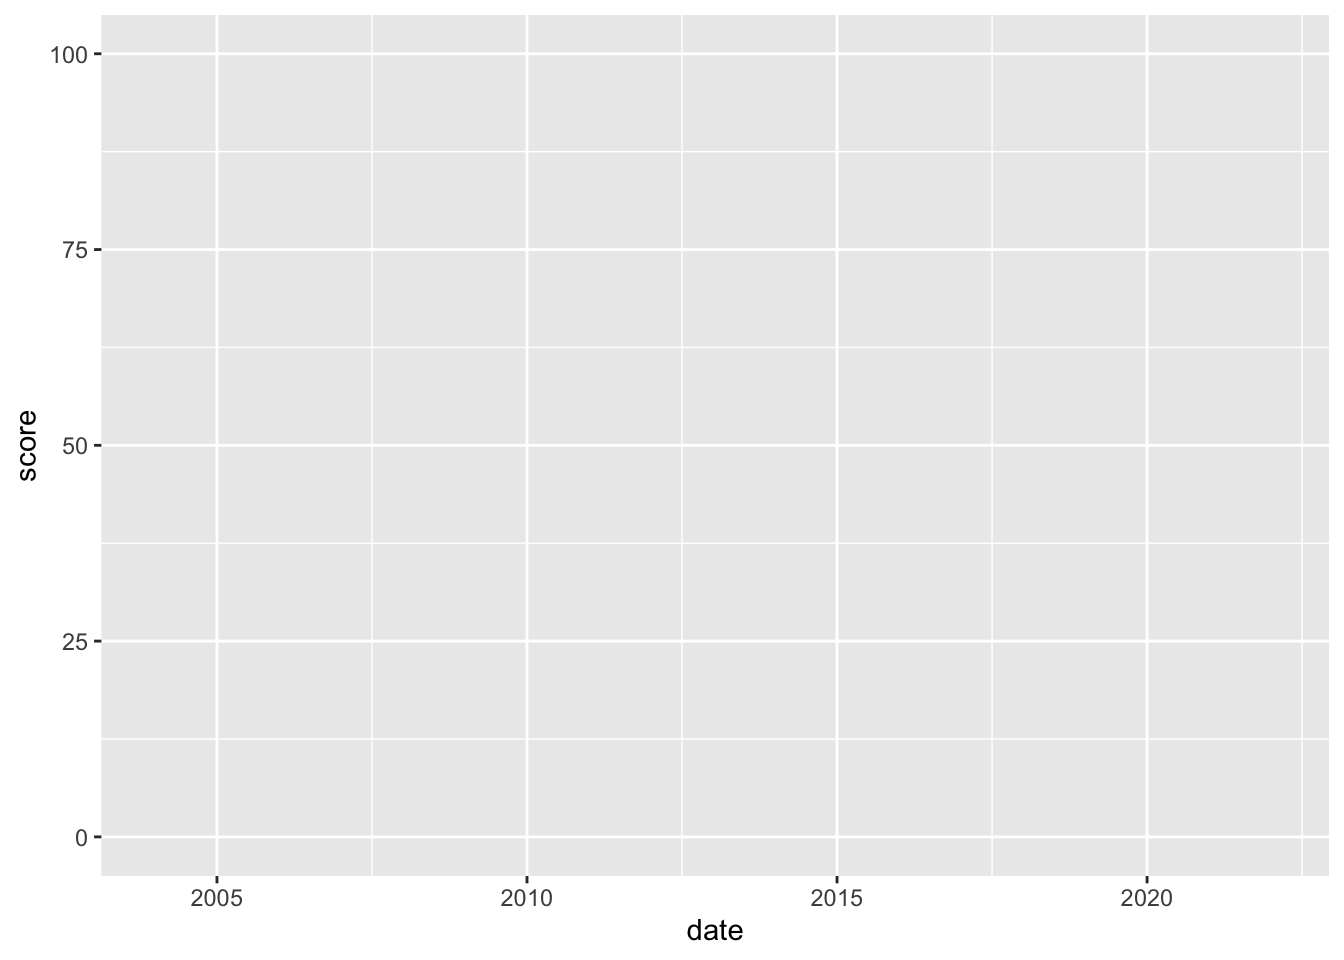
\includegraphics{lecture03---visualization_files/figure-latex/unnamed-chunk-5-1.pdf}

Nothing appears in this graph because we specified the aesthetics but
never specified what to do with them

\begin{Shaded}
\begin{Highlighting}[]
\NormalTok{kard\_tidy }\SpecialCharTok{\%\textgreater{}\%} 
  \FunctionTok{ggplot}\NormalTok{(}\FunctionTok{aes}\NormalTok{(}\AttributeTok{x =}\NormalTok{ date, }\AttributeTok{y =}\NormalTok{ score, }\AttributeTok{color =}\NormalTok{ name)) }\SpecialCharTok{+}
  \FunctionTok{geom\_line}\NormalTok{()}
\end{Highlighting}
\end{Shaded}

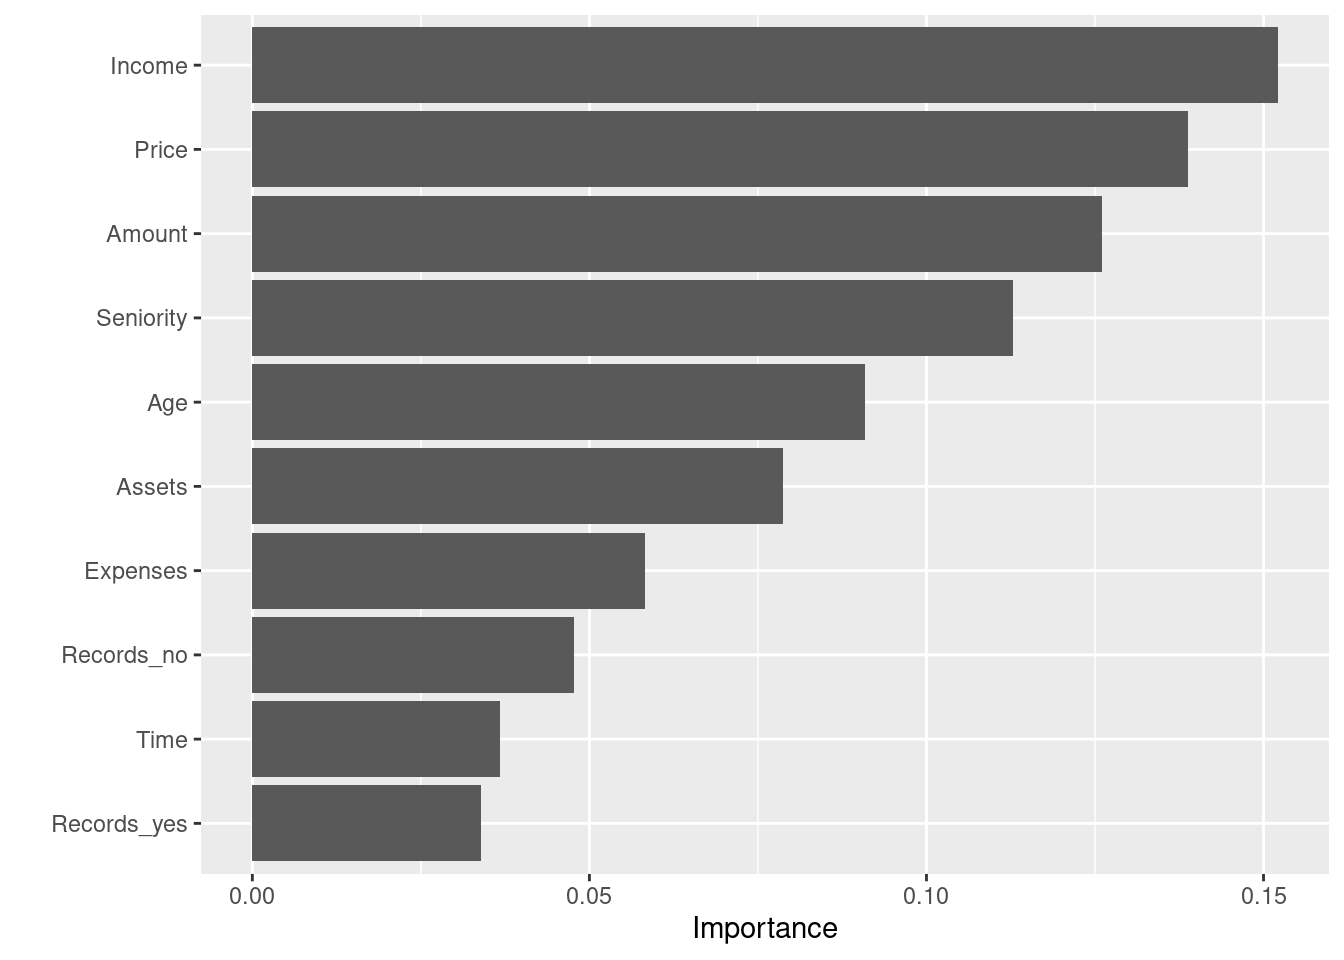
\includegraphics{lecture03---visualization_files/figure-latex/unnamed-chunk-6-1.pdf}

\begin{Shaded}
\begin{Highlighting}[]
\NormalTok{kard\_tidy }\SpecialCharTok{\%\textgreater{}\%} 
  \FunctionTok{ggplot}\NormalTok{(}\FunctionTok{aes}\NormalTok{(}\AttributeTok{x =}\NormalTok{ date, }\AttributeTok{y =}\NormalTok{ score, }\AttributeTok{color =}\NormalTok{ name)) }\SpecialCharTok{+}
  \FunctionTok{geom\_point}\NormalTok{()}
\end{Highlighting}
\end{Shaded}

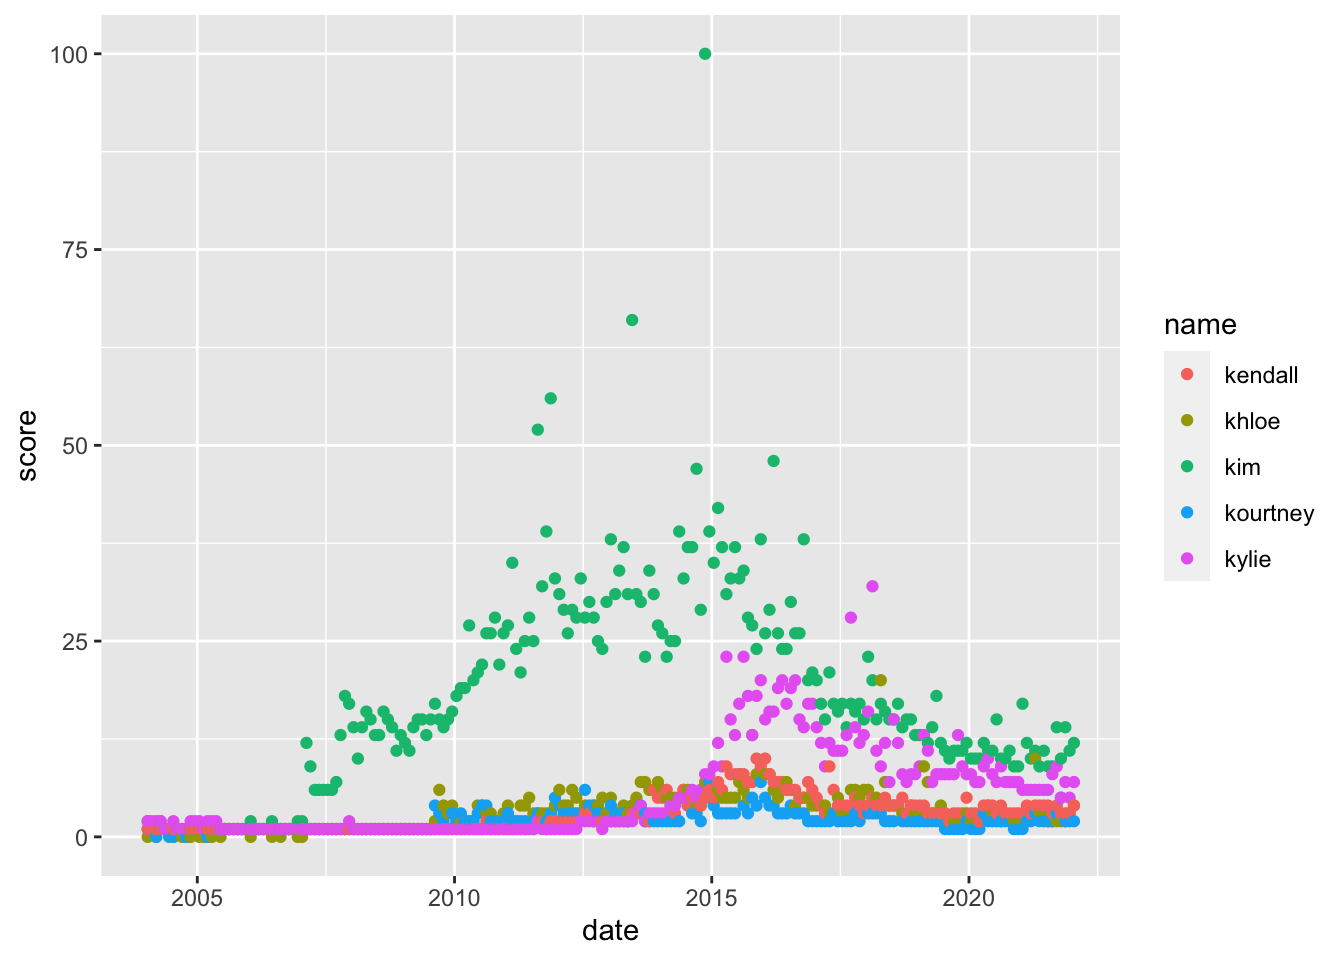
\includegraphics{lecture03---visualization_files/figure-latex/unnamed-chunk-7-1.pdf}

\begin{Shaded}
\begin{Highlighting}[]
\NormalTok{kard\_tidy }\SpecialCharTok{\%\textgreater{}\%} 
  \FunctionTok{ggplot}\NormalTok{(}\FunctionTok{aes}\NormalTok{(}\AttributeTok{x =}\NormalTok{ date, }\AttributeTok{y =}\NormalTok{ score, }\AttributeTok{color =}\NormalTok{ name)) }\SpecialCharTok{+}
  \FunctionTok{geom\_col}\NormalTok{(}\AttributeTok{position =} \StringTok{"dodge"}\NormalTok{)}
\end{Highlighting}
\end{Shaded}

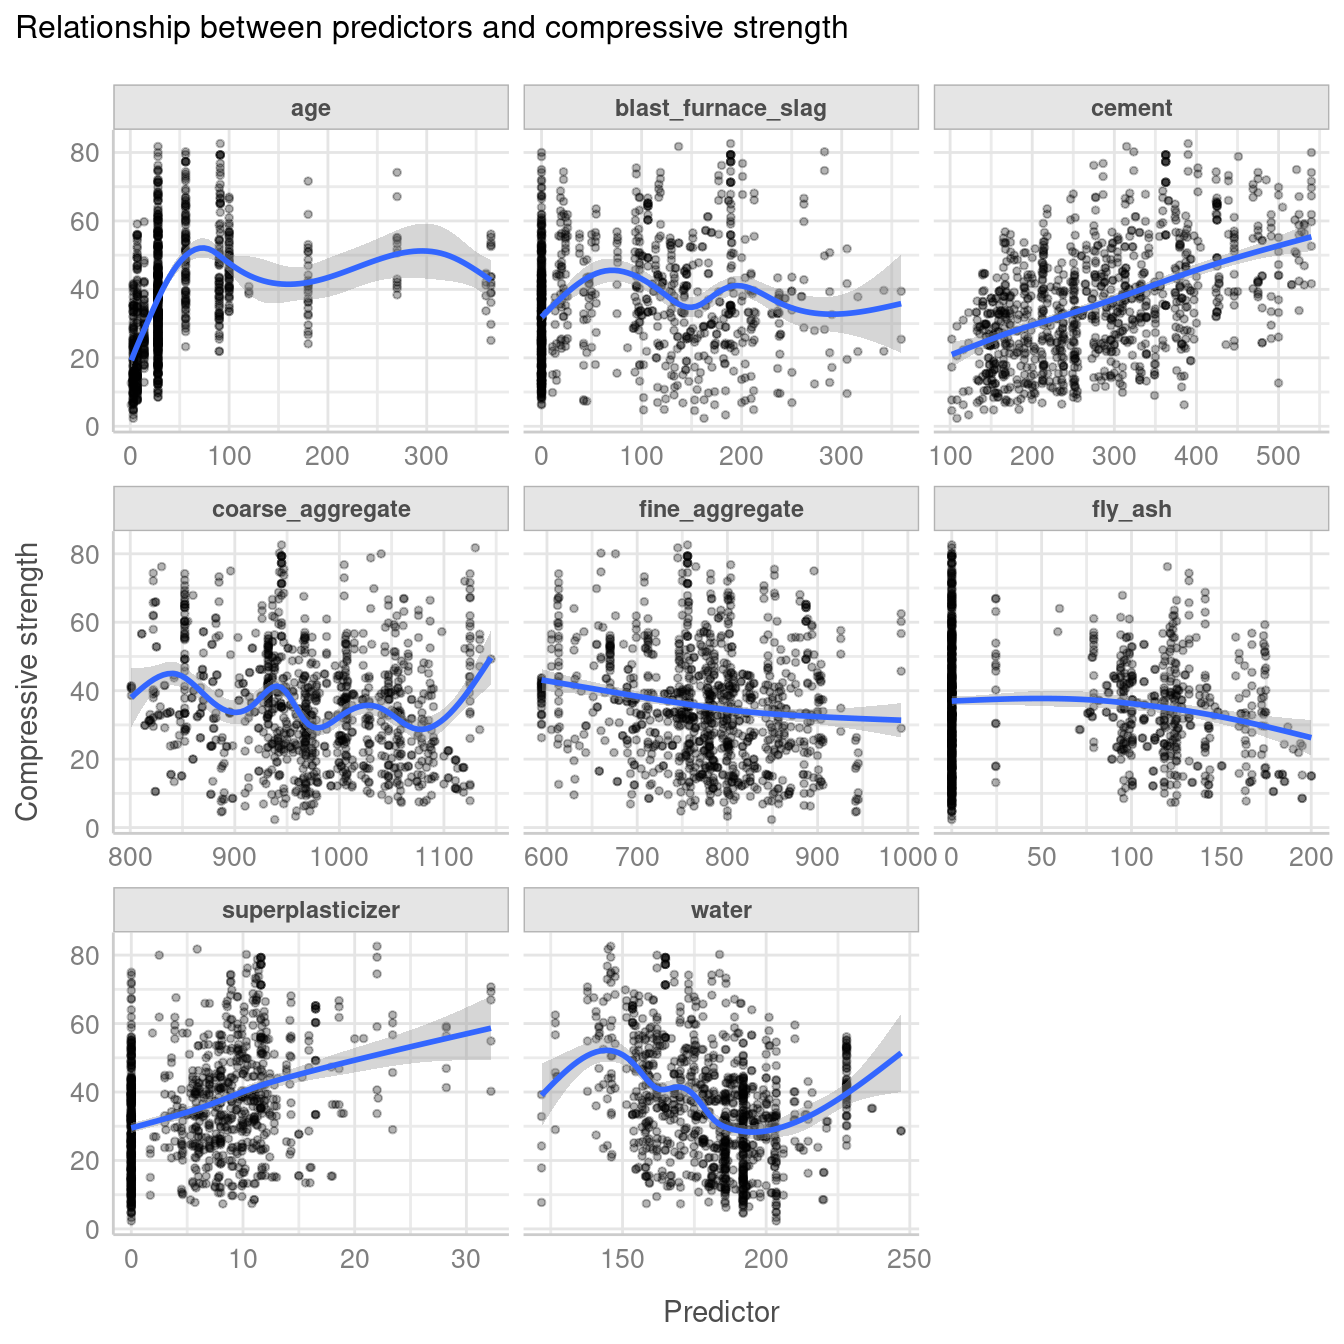
\includegraphics{lecture03---visualization_files/figure-latex/unnamed-chunk-8-1.pdf}

\begin{Shaded}
\begin{Highlighting}[]
\NormalTok{kard\_tidy }\SpecialCharTok{\%\textgreater{}\%} 
  \FunctionTok{ggplot}\NormalTok{(}\FunctionTok{aes}\NormalTok{(}\AttributeTok{x =}\NormalTok{ date, }\AttributeTok{y =}\NormalTok{ score, }\AttributeTok{color =}\NormalTok{ name)) }\SpecialCharTok{+}
  \FunctionTok{geom\_line}\NormalTok{() }\SpecialCharTok{+} 
  \FunctionTok{geom\_smooth}\NormalTok{(}\AttributeTok{method =} \StringTok{"loess"}\NormalTok{)}
\end{Highlighting}
\end{Shaded}

\begin{verbatim}
## `geom_smooth()` using formula 'y ~ x'
\end{verbatim}

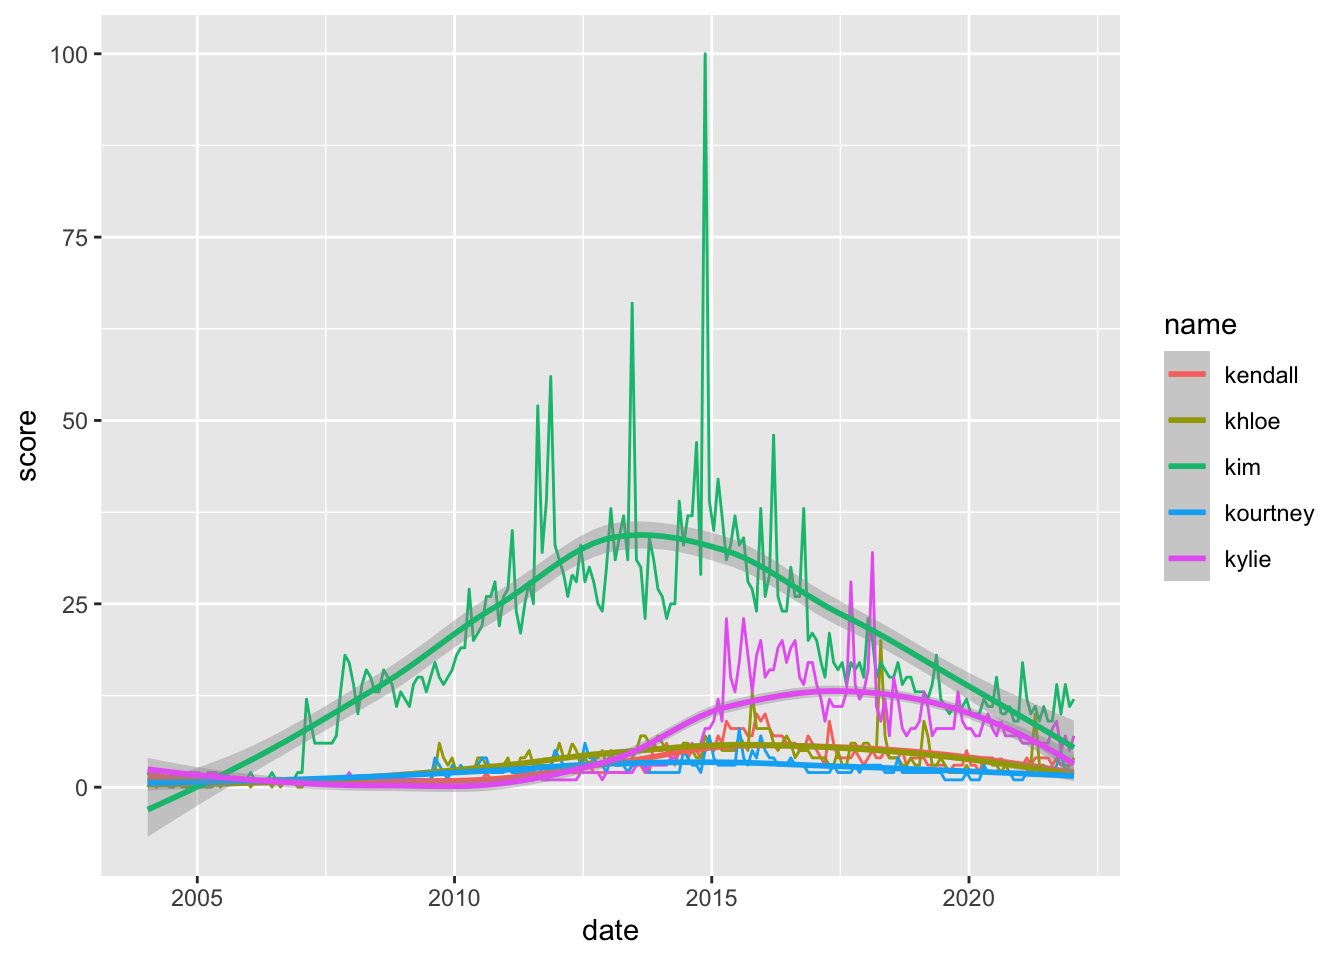
\includegraphics{lecture03---visualization_files/figure-latex/unnamed-chunk-9-1.pdf}

Are they on average growing in popularity or not?

\begin{Shaded}
\begin{Highlighting}[]
\NormalTok{kard\_tidy }\SpecialCharTok{\%\textgreater{}\%} 
  \FunctionTok{ggplot}\NormalTok{(}\FunctionTok{aes}\NormalTok{(}\AttributeTok{x =}\NormalTok{ date, }\AttributeTok{y =}\NormalTok{ score, }\AttributeTok{color =}\NormalTok{ name)) }\SpecialCharTok{+}
  \FunctionTok{geom\_line}\NormalTok{() }\SpecialCharTok{+} 
  \FunctionTok{geom\_smooth}\NormalTok{(}\AttributeTok{method =} \StringTok{"lm"}\NormalTok{)}
\end{Highlighting}
\end{Shaded}

\begin{verbatim}
## `geom_smooth()` using formula 'y ~ x'
\end{verbatim}

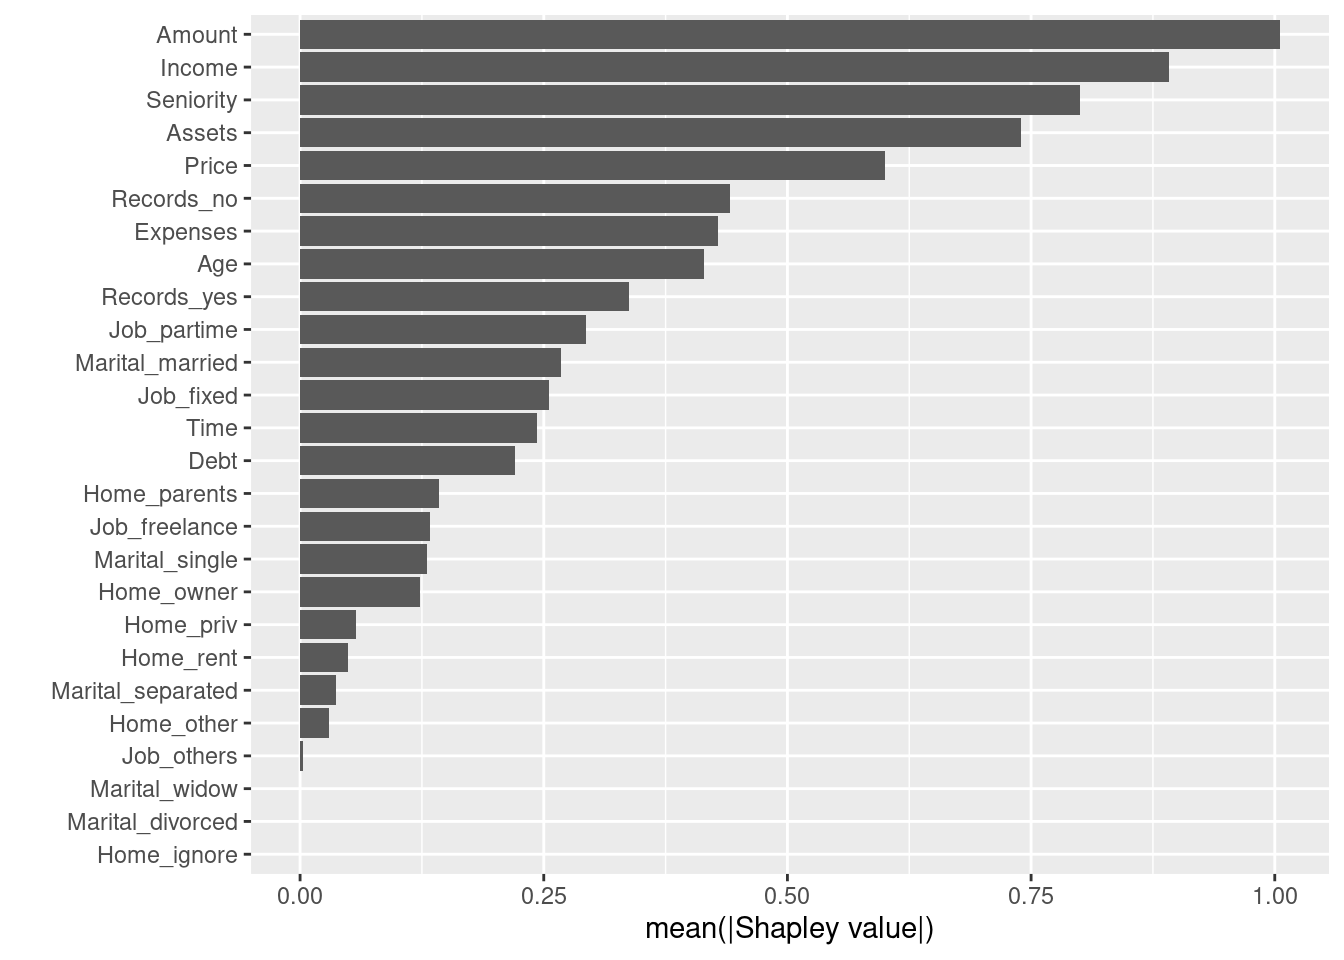
\includegraphics{lecture03---visualization_files/figure-latex/unnamed-chunk-10-1.pdf}

\url{https://www.datanovia.com/en/blog/top-r-color-palettes-to-know-for-great-data-visualization/}
for theme colors

We can modify the coordinate system

\begin{Shaded}
\begin{Highlighting}[]
\NormalTok{kard\_tidy }\SpecialCharTok{\%\textgreater{}\%} 
  \FunctionTok{ggplot}\NormalTok{(}\FunctionTok{aes}\NormalTok{(}\AttributeTok{x =}\NormalTok{ date, }\AttributeTok{y =}\NormalTok{ score, }\AttributeTok{color =}\NormalTok{ name)) }\SpecialCharTok{+}
  \FunctionTok{geom\_line}\NormalTok{() }\SpecialCharTok{+}
  \FunctionTok{scale\_y\_log10}\NormalTok{()}
\end{Highlighting}
\end{Shaded}

\begin{verbatim}
## Warning: Transformation introduced infinite values in continuous y-axis
\end{verbatim}

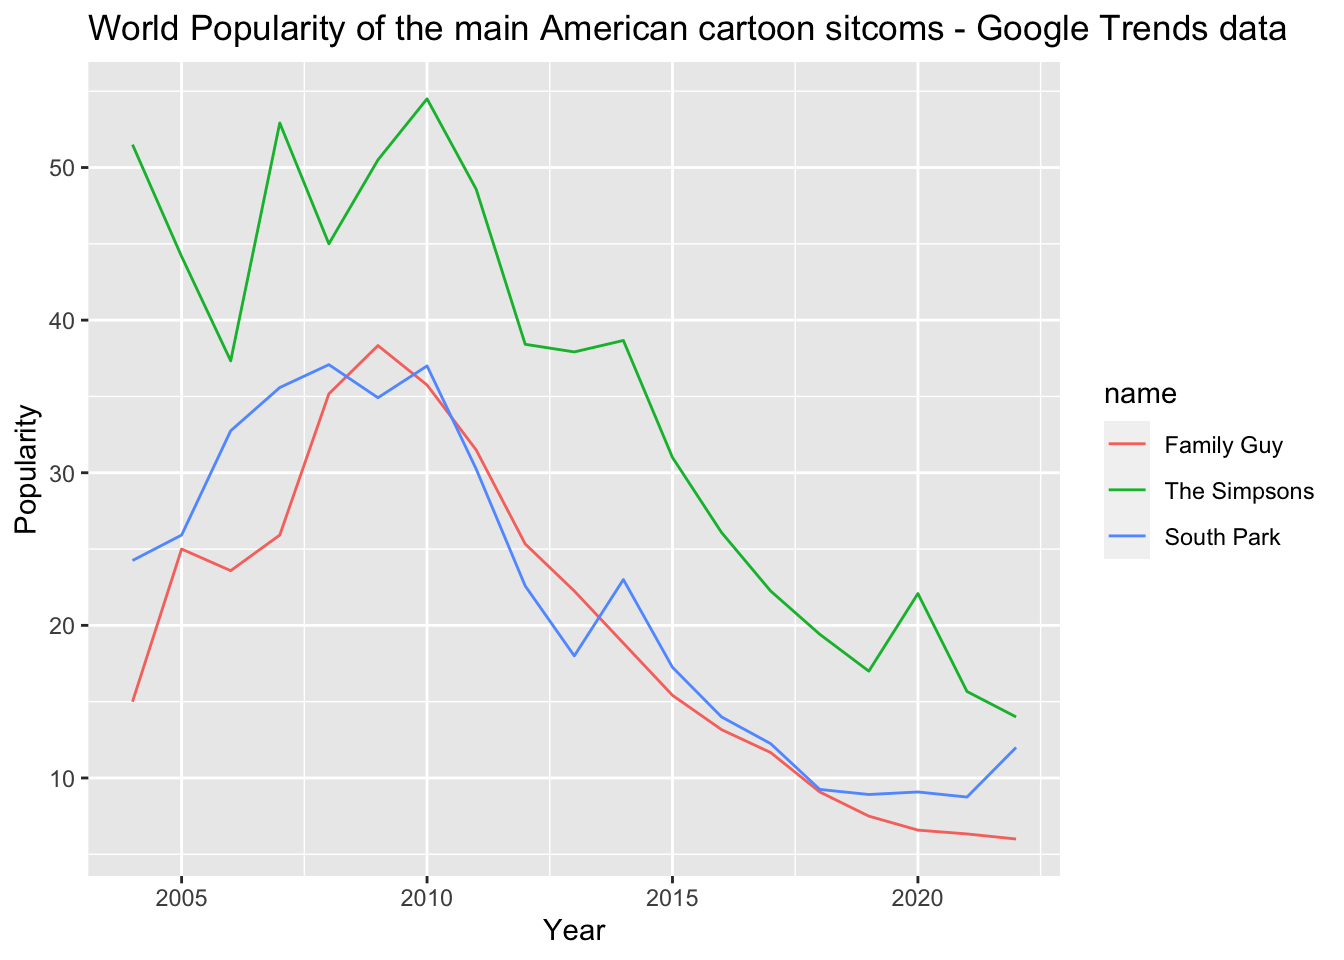
\includegraphics{lecture03---visualization_files/figure-latex/unnamed-chunk-11-1.pdf}

We can also modify the labels

\begin{Shaded}
\begin{Highlighting}[]
\NormalTok{kard\_tidy }\SpecialCharTok{\%\textgreater{}\%} 
  \FunctionTok{ggplot}\NormalTok{(}\FunctionTok{aes}\NormalTok{(}\AttributeTok{x =}\NormalTok{ date, }\AttributeTok{y =}\NormalTok{ score, }\AttributeTok{color =}\NormalTok{ name)) }\SpecialCharTok{+}
  \FunctionTok{geom\_line}\NormalTok{() }\SpecialCharTok{+}
  \FunctionTok{labs}\NormalTok{(}\AttributeTok{x =} \StringTok{"Date"}\NormalTok{,}
       \AttributeTok{y =} \StringTok{"Popularity"}\NormalTok{,}
       \AttributeTok{title =} \StringTok{"The Popularity of the Kardashians, Google Trends data"}\NormalTok{,}
\NormalTok{       )}
\end{Highlighting}
\end{Shaded}

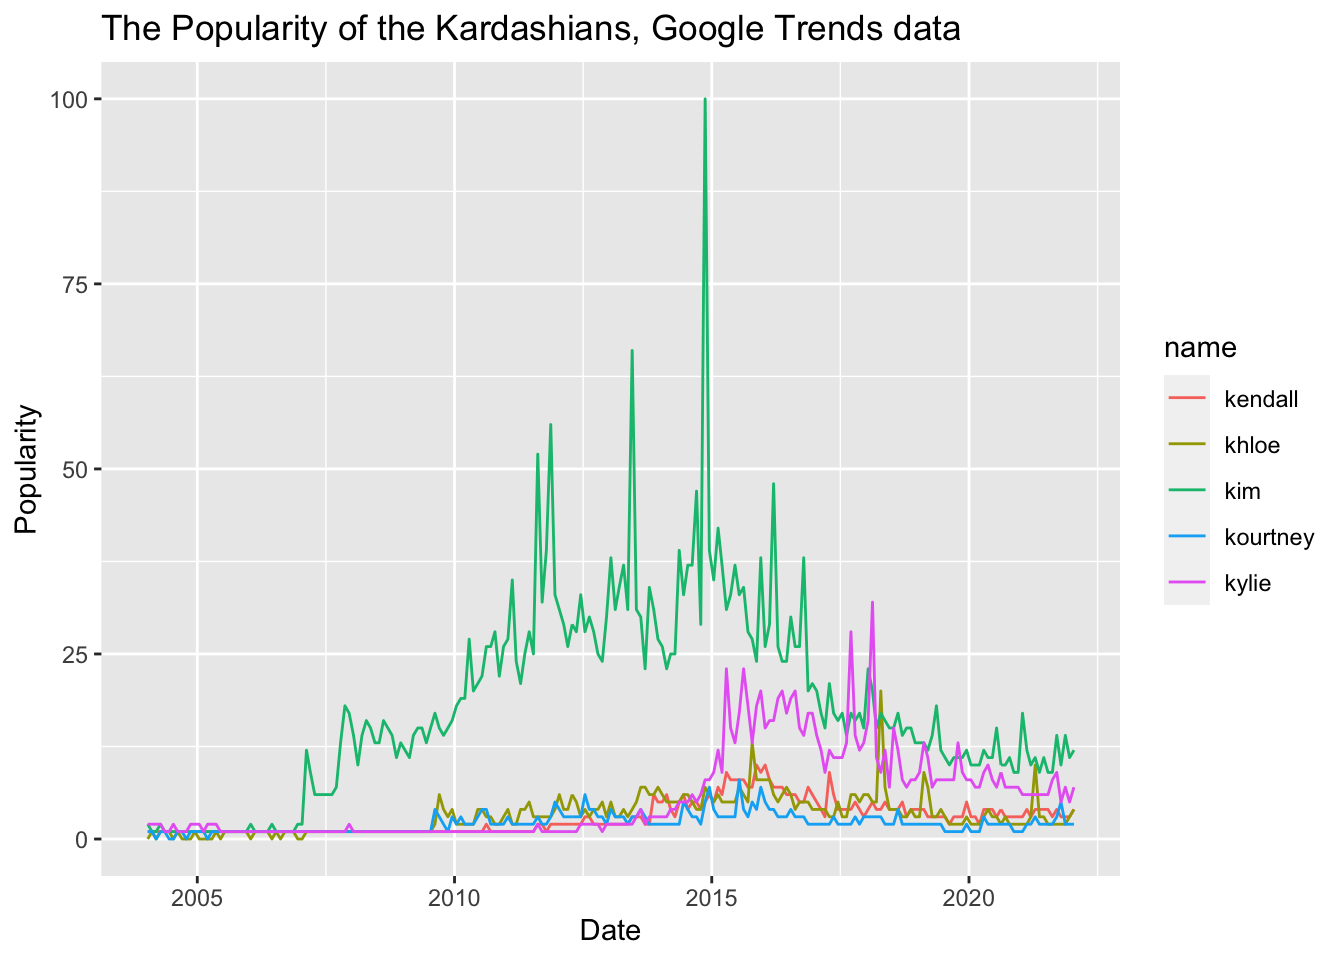
\includegraphics{lecture03---visualization_files/figure-latex/unnamed-chunk-12-1.pdf}

We can also modify the legend text

\begin{Shaded}
\begin{Highlighting}[]
\NormalTok{kard\_tidy }\SpecialCharTok{\%\textgreater{}\%} 
  \FunctionTok{ggplot}\NormalTok{(}\FunctionTok{aes}\NormalTok{(}\AttributeTok{x =}\NormalTok{ date, }\AttributeTok{y =}\NormalTok{ score, }\AttributeTok{color =}\NormalTok{ name)) }\SpecialCharTok{+}
  \FunctionTok{geom\_line}\NormalTok{() }\SpecialCharTok{+}
  \FunctionTok{labs}\NormalTok{(}\AttributeTok{x =} \StringTok{"Date"}\NormalTok{,}
       \AttributeTok{y =} \StringTok{"Popularity"}\NormalTok{,}
       \AttributeTok{title =} \StringTok{"The Popularity of the Kardashians, Google Trends data"}\NormalTok{,}
\NormalTok{       ) }\SpecialCharTok{+}
  \FunctionTok{scale\_color\_discrete}\NormalTok{(}\AttributeTok{name =} \StringTok{"Name"}\NormalTok{,}
                       \AttributeTok{labels =} \FunctionTok{c}\NormalTok{(}\StringTok{"Kendall"}\NormalTok{, }\StringTok{"Khloe"}\NormalTok{, }\StringTok{"Kim"}\NormalTok{, }\StringTok{"Kourtney"}\NormalTok{, }\StringTok{"Kylie"}\NormalTok{))}
\end{Highlighting}
\end{Shaded}

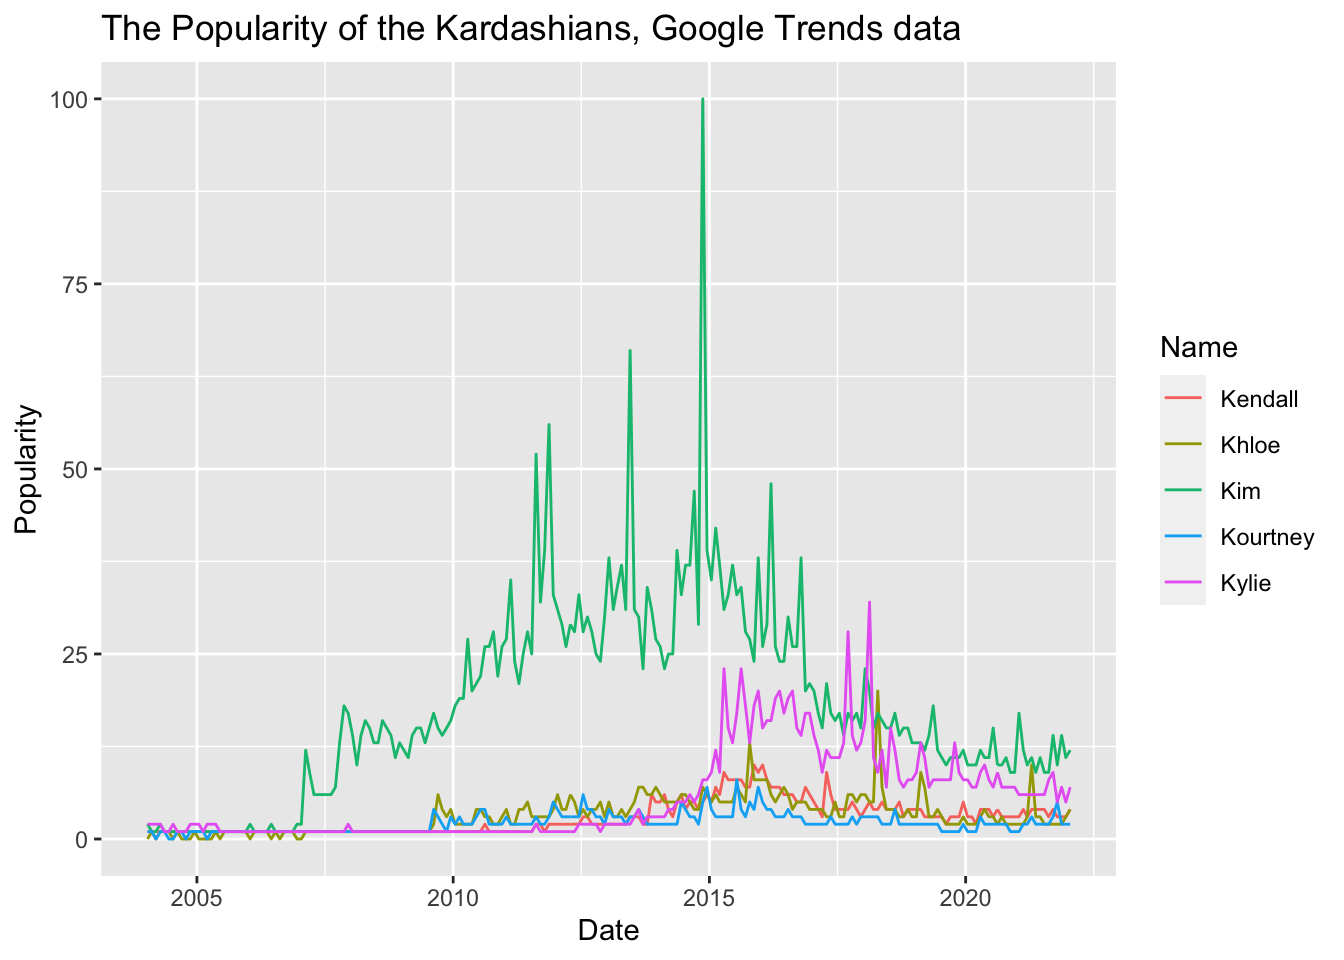
\includegraphics{lecture03---visualization_files/figure-latex/unnamed-chunk-13-1.pdf}

The grey background is not the most aesthetically pleasing so we can
remove it:

\begin{Shaded}
\begin{Highlighting}[]
\NormalTok{kard\_tidy }\SpecialCharTok{\%\textgreater{}\%} 
  \FunctionTok{ggplot}\NormalTok{(}\FunctionTok{aes}\NormalTok{(}\AttributeTok{x =}\NormalTok{ date, }\AttributeTok{y =}\NormalTok{ score, }\AttributeTok{color =}\NormalTok{ name)) }\SpecialCharTok{+}
  \FunctionTok{geom\_line}\NormalTok{() }\SpecialCharTok{+}
  \FunctionTok{labs}\NormalTok{(}\AttributeTok{x =} \StringTok{"Date"}\NormalTok{,}
       \AttributeTok{y =} \StringTok{"Popularity"}\NormalTok{,}
       \AttributeTok{title =} \StringTok{"The Popularity of the Kardashians, Google Trends data"}\NormalTok{,}
\NormalTok{       ) }\SpecialCharTok{+}
  \FunctionTok{scale\_color\_discrete}\NormalTok{(}\AttributeTok{name =} \StringTok{"Name"}\NormalTok{,}
                       \AttributeTok{labels =} \FunctionTok{c}\NormalTok{(}\StringTok{"Kendall"}\NormalTok{, }\StringTok{"Khloe"}\NormalTok{, }\StringTok{"Kim"}\NormalTok{, }\StringTok{"Kourtney"}\NormalTok{, }\StringTok{"Kylie"}\NormalTok{)) }\SpecialCharTok{+}
  \FunctionTok{theme\_classic}\NormalTok{()}
\end{Highlighting}
\end{Shaded}

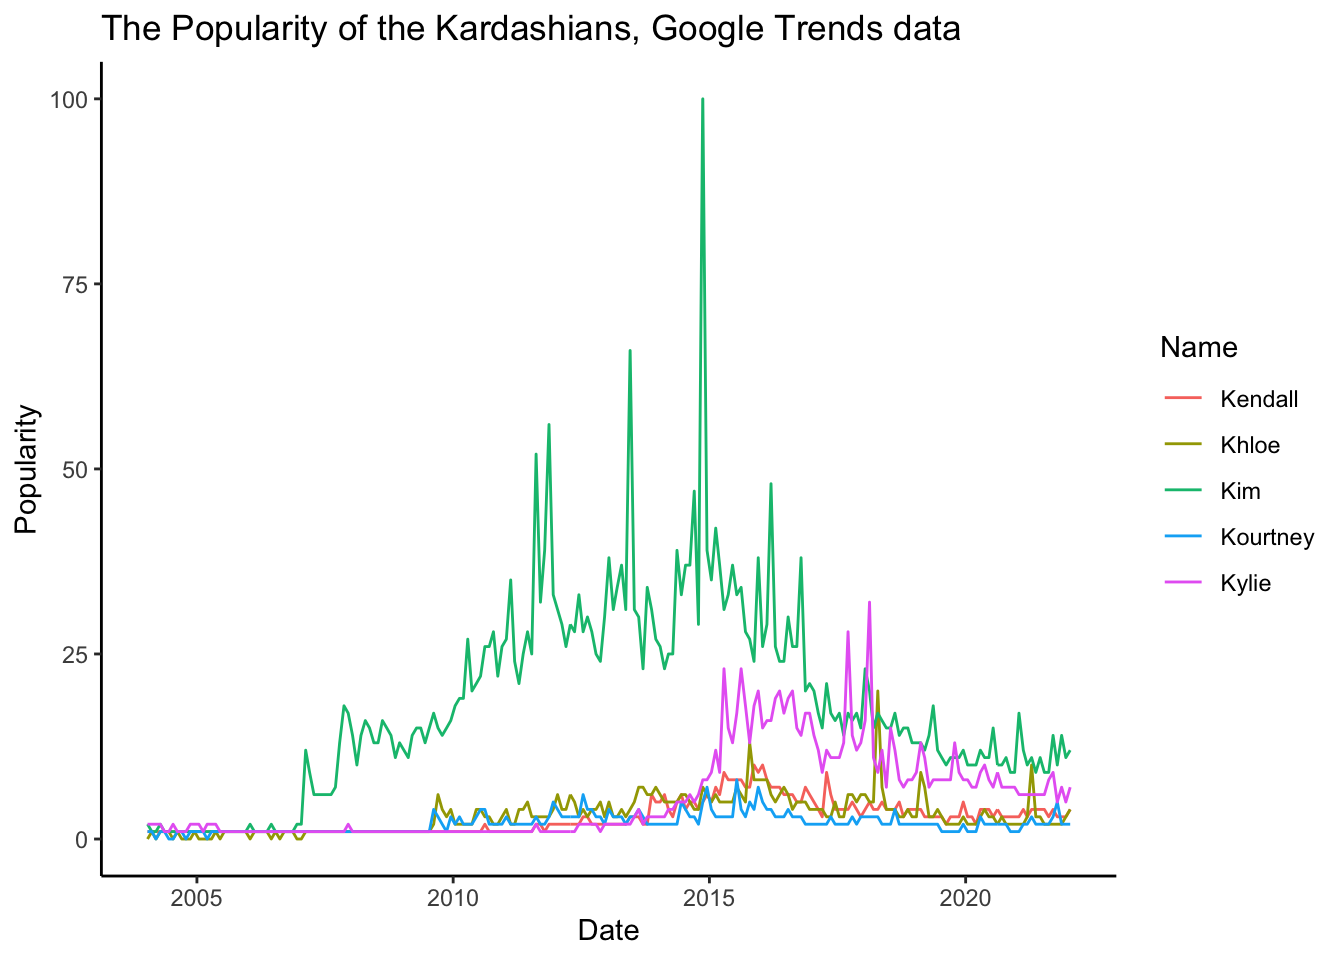
\includegraphics{lecture03---visualization_files/figure-latex/unnamed-chunk-14-1.pdf}

There are a lot of cool themes inside \texttt{ggthemes}

\begin{Shaded}
\begin{Highlighting}[]
\NormalTok{kard\_tidy }\SpecialCharTok{\%\textgreater{}\%} 
  \FunctionTok{ggplot}\NormalTok{(}\FunctionTok{aes}\NormalTok{(}\AttributeTok{x =}\NormalTok{ date, }\AttributeTok{y =}\NormalTok{ score, }\AttributeTok{color =}\NormalTok{ name)) }\SpecialCharTok{+}
  \FunctionTok{geom\_line}\NormalTok{() }\SpecialCharTok{+}
  \FunctionTok{labs}\NormalTok{(}\AttributeTok{x =} \StringTok{"Date"}\NormalTok{,}
       \AttributeTok{y =} \StringTok{"Popularity"}\NormalTok{,}
       \AttributeTok{title =} \StringTok{"The Popularity of the Kardashians, Google Trends data"}\NormalTok{,}
\NormalTok{       ) }\SpecialCharTok{+}
  \FunctionTok{scale\_color\_discrete}\NormalTok{(}\AttributeTok{name =} \StringTok{"Name"}\NormalTok{,}
                       \AttributeTok{labels =} \FunctionTok{c}\NormalTok{(}\StringTok{"Kendall"}\NormalTok{, }\StringTok{"Khloe"}\NormalTok{, }\StringTok{"Kim"}\NormalTok{, }\StringTok{"Kourtney"}\NormalTok{, }\StringTok{"Kylie"}\NormalTok{)) }\SpecialCharTok{+}
  \FunctionTok{theme\_wsj}\NormalTok{()}
\end{Highlighting}
\end{Shaded}

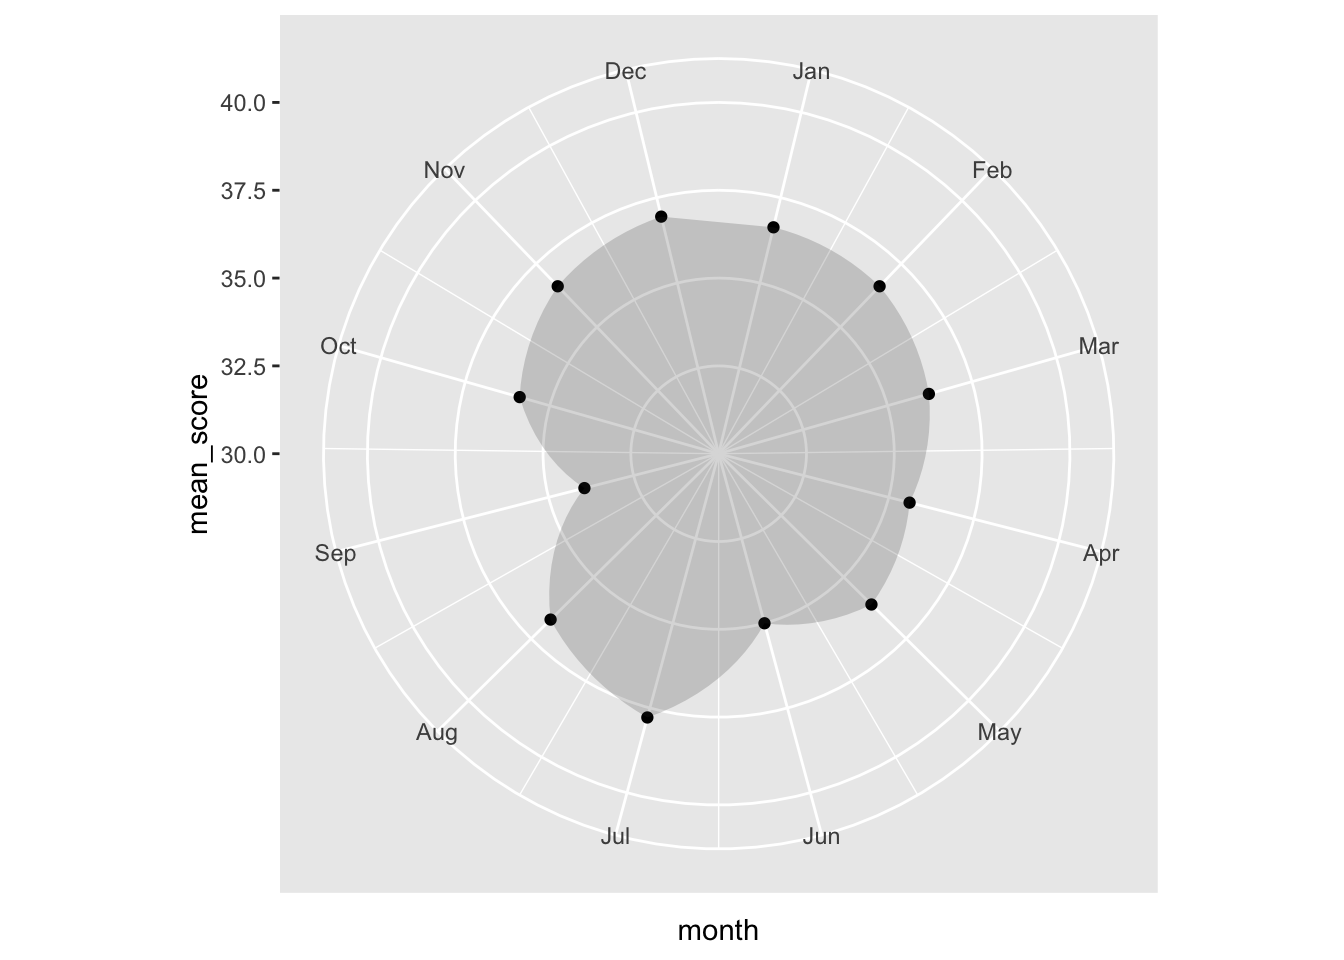
\includegraphics{lecture03---visualization_files/figure-latex/unnamed-chunk-15-1.pdf}

Let's fix the title since it doesn't display properly

\begin{Shaded}
\begin{Highlighting}[]
\NormalTok{kard\_tidy }\SpecialCharTok{\%\textgreater{}\%} 
  \FunctionTok{ggplot}\NormalTok{(}\FunctionTok{aes}\NormalTok{(}\AttributeTok{x =}\NormalTok{ date, }\AttributeTok{y =}\NormalTok{ score, }\AttributeTok{color =}\NormalTok{ name)) }\SpecialCharTok{+}
  \FunctionTok{geom\_line}\NormalTok{() }\SpecialCharTok{+}
  \FunctionTok{labs}\NormalTok{(}\AttributeTok{x =} \StringTok{"Date"}\NormalTok{,}
       \AttributeTok{y =} \StringTok{"Popularity"}\NormalTok{,}
       \AttributeTok{title =} \StringTok{"The Popularity of the }\SpecialCharTok{\textbackslash{}n}\StringTok{ Kardashians"}\NormalTok{,}
       \AttributeTok{subtitle =} \StringTok{"Google trends data"}
\NormalTok{       ) }\SpecialCharTok{+}
  \FunctionTok{scale\_color\_discrete}\NormalTok{(}\AttributeTok{name =} \StringTok{"Name"}\NormalTok{,}
                       \AttributeTok{labels =} \FunctionTok{c}\NormalTok{(}\StringTok{"Kendall"}\NormalTok{, }\StringTok{"Khloe"}\NormalTok{, }\StringTok{"Kim"}\NormalTok{, }\StringTok{"Kourtney"}\NormalTok{, }\StringTok{"Kylie"}\NormalTok{)) }\SpecialCharTok{+}
  \FunctionTok{theme\_wsj}\NormalTok{()}
\end{Highlighting}
\end{Shaded}

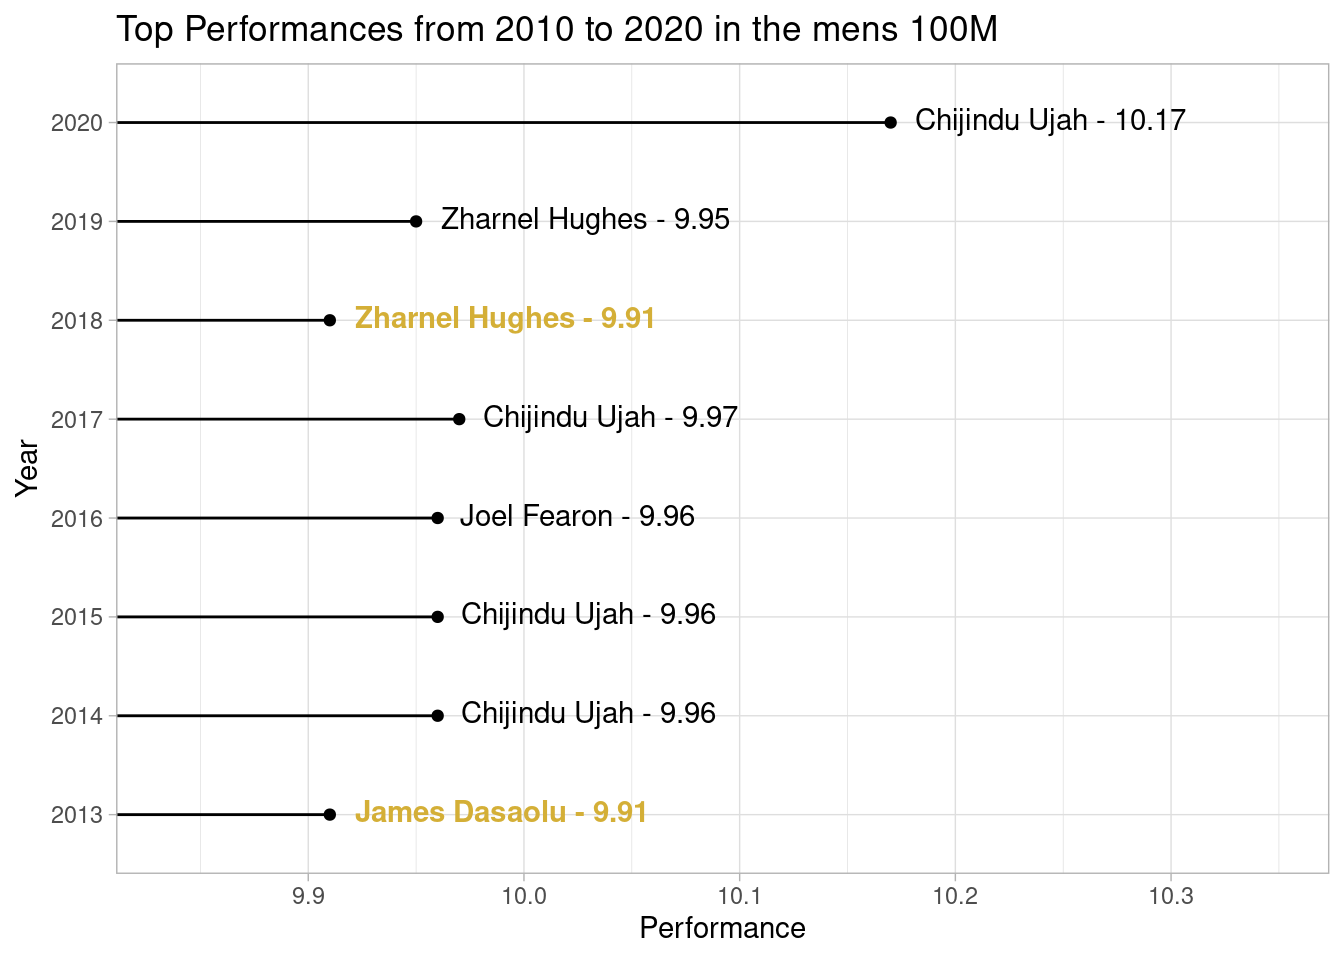
\includegraphics{lecture03---visualization_files/figure-latex/unnamed-chunk-16-1.pdf}

\begin{Shaded}
\begin{Highlighting}[]
\NormalTok{kard\_tidy }\SpecialCharTok{\%\textgreater{}\%} 
  \FunctionTok{ggplot}\NormalTok{(}\FunctionTok{aes}\NormalTok{(}\AttributeTok{x =}\NormalTok{ date, }\AttributeTok{y =}\NormalTok{ score, }\AttributeTok{color =}\NormalTok{ name)) }\SpecialCharTok{+}
  \FunctionTok{geom\_line}\NormalTok{() }\SpecialCharTok{+}
  \FunctionTok{labs}\NormalTok{(}\AttributeTok{x =} \StringTok{"Date"}\NormalTok{,}
       \AttributeTok{y =} \StringTok{"Popularity"}\NormalTok{,}
       \AttributeTok{title =} \StringTok{"The Popularity of the Kardashians"}\NormalTok{,}
       \AttributeTok{subtitle =} \StringTok{"Google trends data"}
\NormalTok{       ) }\SpecialCharTok{+}
  \FunctionTok{scale\_color\_discrete}\NormalTok{(}\AttributeTok{name =} \StringTok{"Name"}\NormalTok{,}
                       \AttributeTok{labels =} \FunctionTok{c}\NormalTok{(}\StringTok{"Kendall"}\NormalTok{, }\StringTok{"Khloe"}\NormalTok{, }\StringTok{"Kim"}\NormalTok{, }\StringTok{"Kourtney"}\NormalTok{, }\StringTok{"Kylie"}\NormalTok{)) }\SpecialCharTok{+}
  \FunctionTok{theme\_economist}\NormalTok{()}
\end{Highlighting}
\end{Shaded}

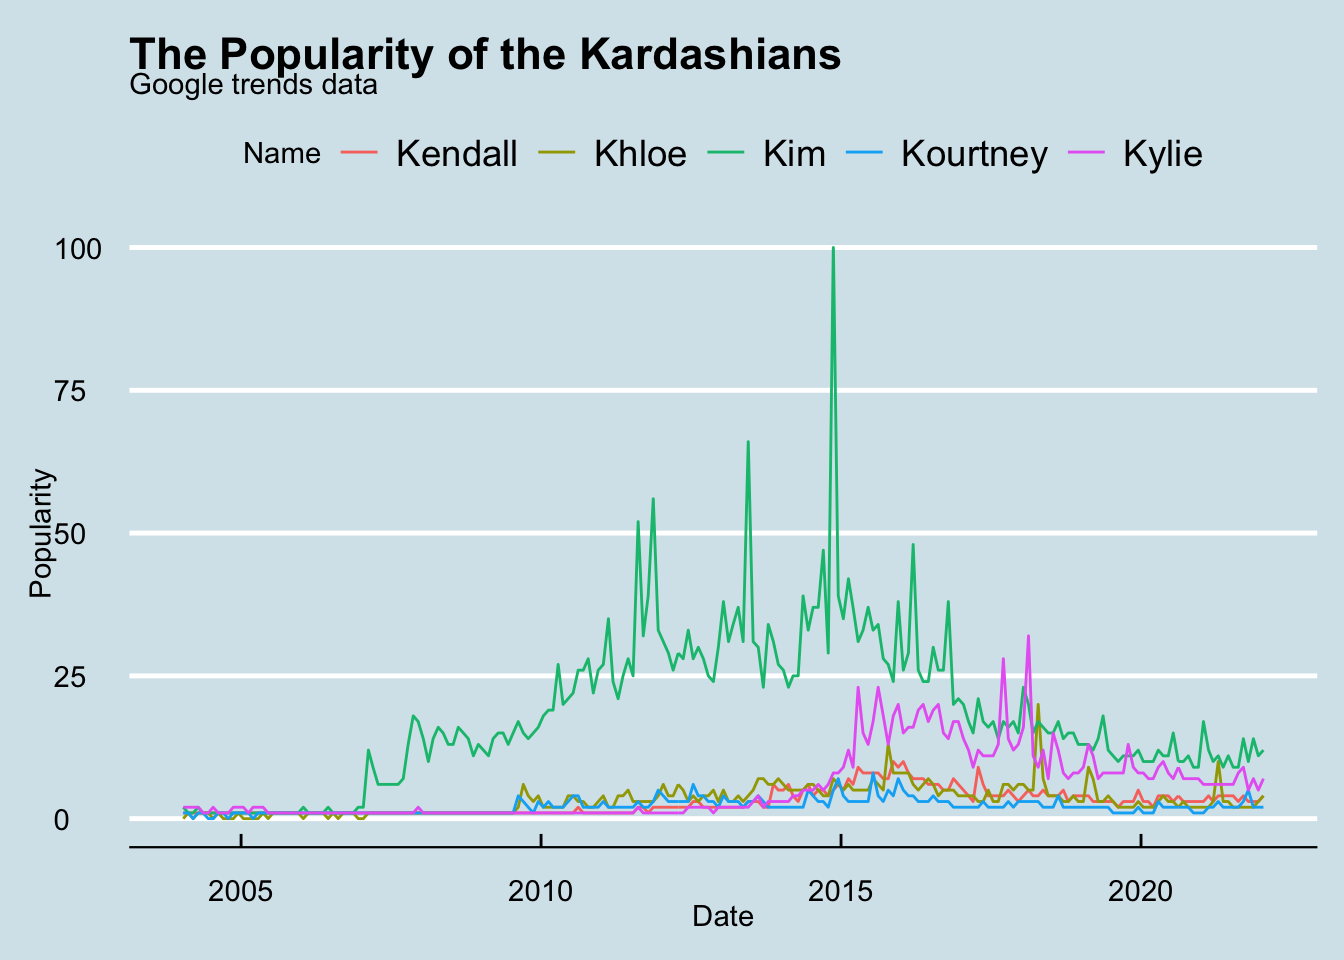
\includegraphics{lecture03---visualization_files/figure-latex/unnamed-chunk-17-1.pdf}

We might want to change the colors of the lines now

\begin{Shaded}
\begin{Highlighting}[]
\NormalTok{kard\_tidy }\SpecialCharTok{\%\textgreater{}\%} 
  \FunctionTok{ggplot}\NormalTok{(}\FunctionTok{aes}\NormalTok{(}\AttributeTok{x =}\NormalTok{ date, }\AttributeTok{y =}\NormalTok{ score, }\AttributeTok{color =}\NormalTok{ name)) }\SpecialCharTok{+}
  \FunctionTok{geom\_line}\NormalTok{() }\SpecialCharTok{+}
  \FunctionTok{labs}\NormalTok{(}\AttributeTok{x =} \StringTok{"Date"}\NormalTok{,}
       \AttributeTok{y =} \StringTok{"Popularity"}\NormalTok{,}
       \AttributeTok{title =} \StringTok{"The Popularity of the Kardashians"}\NormalTok{,}
       \AttributeTok{subtitle =} \StringTok{"Google trends data"}
\NormalTok{       ) }\SpecialCharTok{+}
  \FunctionTok{scale\_color\_viridis\_d}\NormalTok{(}\AttributeTok{name =} \StringTok{"Name"}\NormalTok{,}
                       \AttributeTok{labels =} \FunctionTok{c}\NormalTok{(}\StringTok{"Kendall"}\NormalTok{, }\StringTok{"Khloe"}\NormalTok{, }\StringTok{"Kim"}\NormalTok{, }\StringTok{"Kourtney"}\NormalTok{, }\StringTok{"Kylie"}\NormalTok{),}
                       \AttributeTok{option =} \StringTok{"D"}\NormalTok{) }\SpecialCharTok{+}
  \FunctionTok{theme\_economist}\NormalTok{()}
\end{Highlighting}
\end{Shaded}

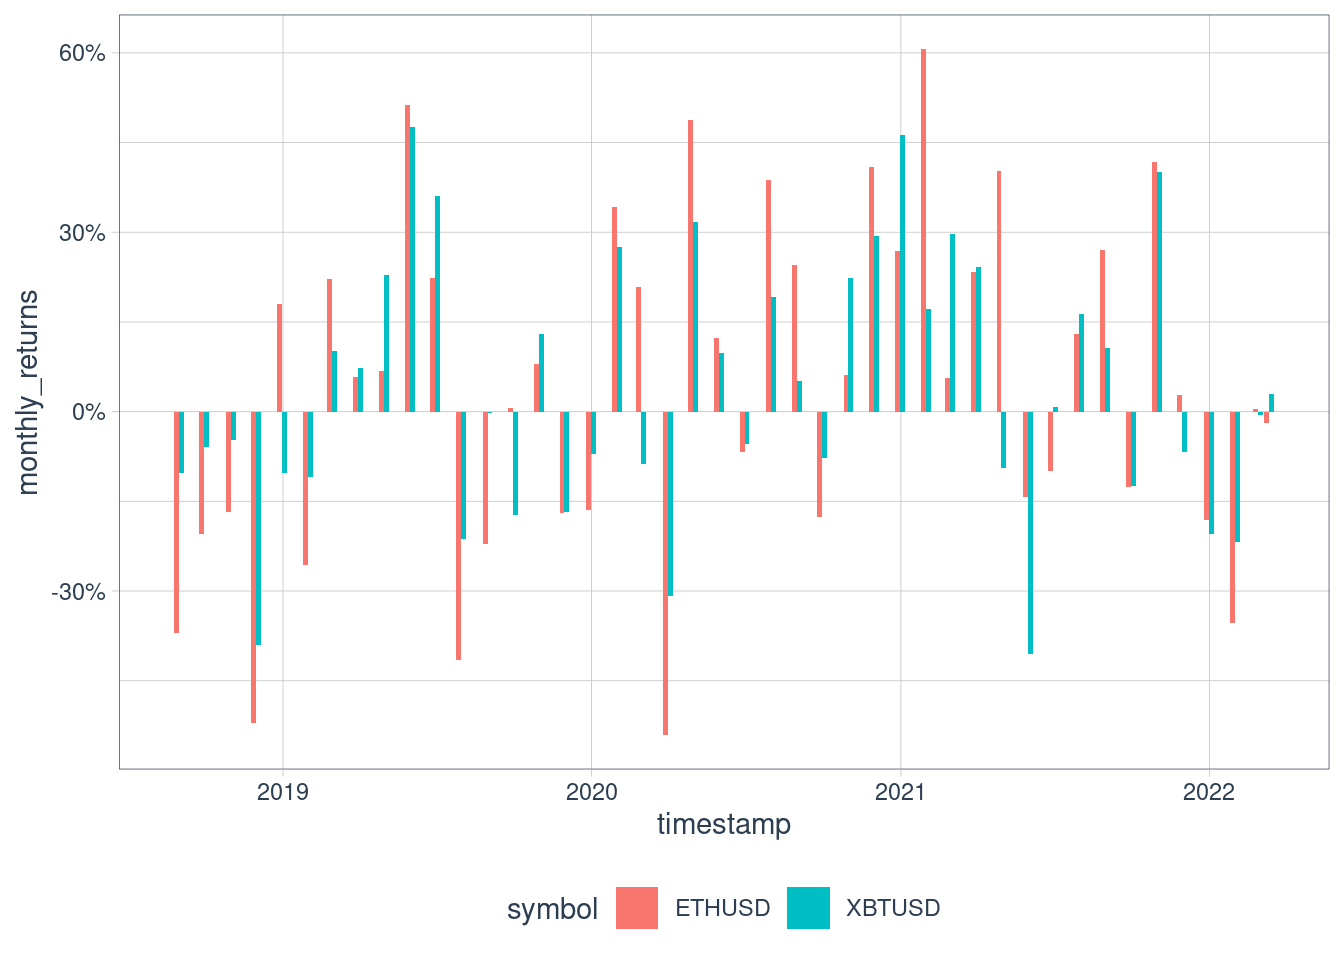
\includegraphics{lecture03---visualization_files/figure-latex/unnamed-chunk-18-1.pdf}

\begin{Shaded}
\begin{Highlighting}[]
\NormalTok{kard\_tidy }\SpecialCharTok{\%\textgreater{}\%} 
  \FunctionTok{ggplot}\NormalTok{(}\FunctionTok{aes}\NormalTok{(}\AttributeTok{x =}\NormalTok{ date, }\AttributeTok{y =}\NormalTok{ score, }\AttributeTok{color =}\NormalTok{ name)) }\SpecialCharTok{+}
  \FunctionTok{geom\_line}\NormalTok{() }\SpecialCharTok{+}
  \FunctionTok{labs}\NormalTok{(}\AttributeTok{x =} \StringTok{"Date"}\NormalTok{,}
       \AttributeTok{y =} \StringTok{"Popularity"}\NormalTok{,}
       \AttributeTok{title =} \StringTok{"The Popularity of the Kardashians"}\NormalTok{,}
       \AttributeTok{subtitle =} \StringTok{"Google trends data"}
\NormalTok{       ) }\SpecialCharTok{+}
  \FunctionTok{scale\_color\_brewer}\NormalTok{(}\AttributeTok{name =} \StringTok{"Name"}\NormalTok{,}
                     \AttributeTok{labels =} \FunctionTok{c}\NormalTok{(}\StringTok{"Kendall"}\NormalTok{, }\StringTok{"Khloe"}\NormalTok{, }\StringTok{"Kim"}\NormalTok{, }\StringTok{"Kourtney"}\NormalTok{, }\StringTok{"Kylie"}\NormalTok{),}
                     \AttributeTok{type =} \StringTok{"qual"}
\NormalTok{                       ) }\SpecialCharTok{+}
  \FunctionTok{theme\_classic}\NormalTok{()}
\end{Highlighting}
\end{Shaded}

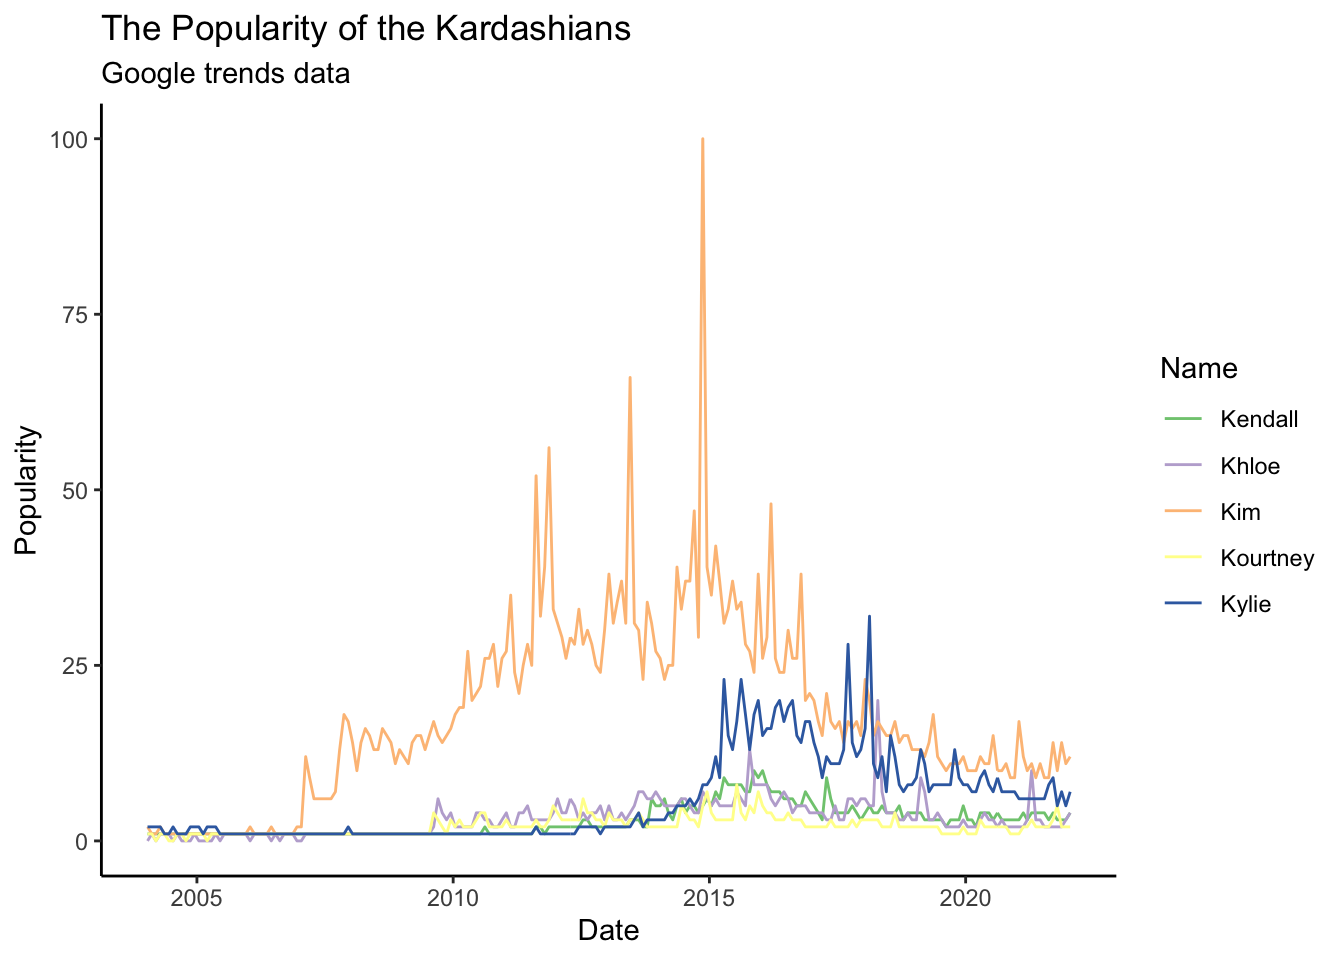
\includegraphics{lecture03---visualization_files/figure-latex/unnamed-chunk-19-1.pdf}

\begin{Shaded}
\begin{Highlighting}[]
\NormalTok{kard\_tidy }\SpecialCharTok{\%\textgreater{}\%} 
  \FunctionTok{ggplot}\NormalTok{(}\FunctionTok{aes}\NormalTok{(}\AttributeTok{x =}\NormalTok{ date, }\AttributeTok{y =}\NormalTok{ score, }\AttributeTok{color =}\NormalTok{ name)) }\SpecialCharTok{+}
  \FunctionTok{geom\_line}\NormalTok{() }\SpecialCharTok{+}
  \FunctionTok{labs}\NormalTok{(}\AttributeTok{x =} \StringTok{"Date"}\NormalTok{,}
       \AttributeTok{y =} \StringTok{"Popularity"}\NormalTok{,}
       \AttributeTok{title =} \StringTok{"The Popularity of the Kardashians"}\NormalTok{,}
       \AttributeTok{subtitle =} \StringTok{"Google trends data"}
\NormalTok{       ) }\SpecialCharTok{+}
  \FunctionTok{scale\_color\_lancet}\NormalTok{(}\AttributeTok{name =} \StringTok{"Name"}\NormalTok{,}
                     \AttributeTok{labels =} \FunctionTok{c}\NormalTok{(}\StringTok{"Kendall"}\NormalTok{, }\StringTok{"Khloe"}\NormalTok{, }\StringTok{"Kim"}\NormalTok{, }\StringTok{"Kourtney"}\NormalTok{, }\StringTok{"Kylie"}\NormalTok{)}
\NormalTok{                       ) }\SpecialCharTok{+}
  \FunctionTok{theme\_classic}\NormalTok{()}
\end{Highlighting}
\end{Shaded}

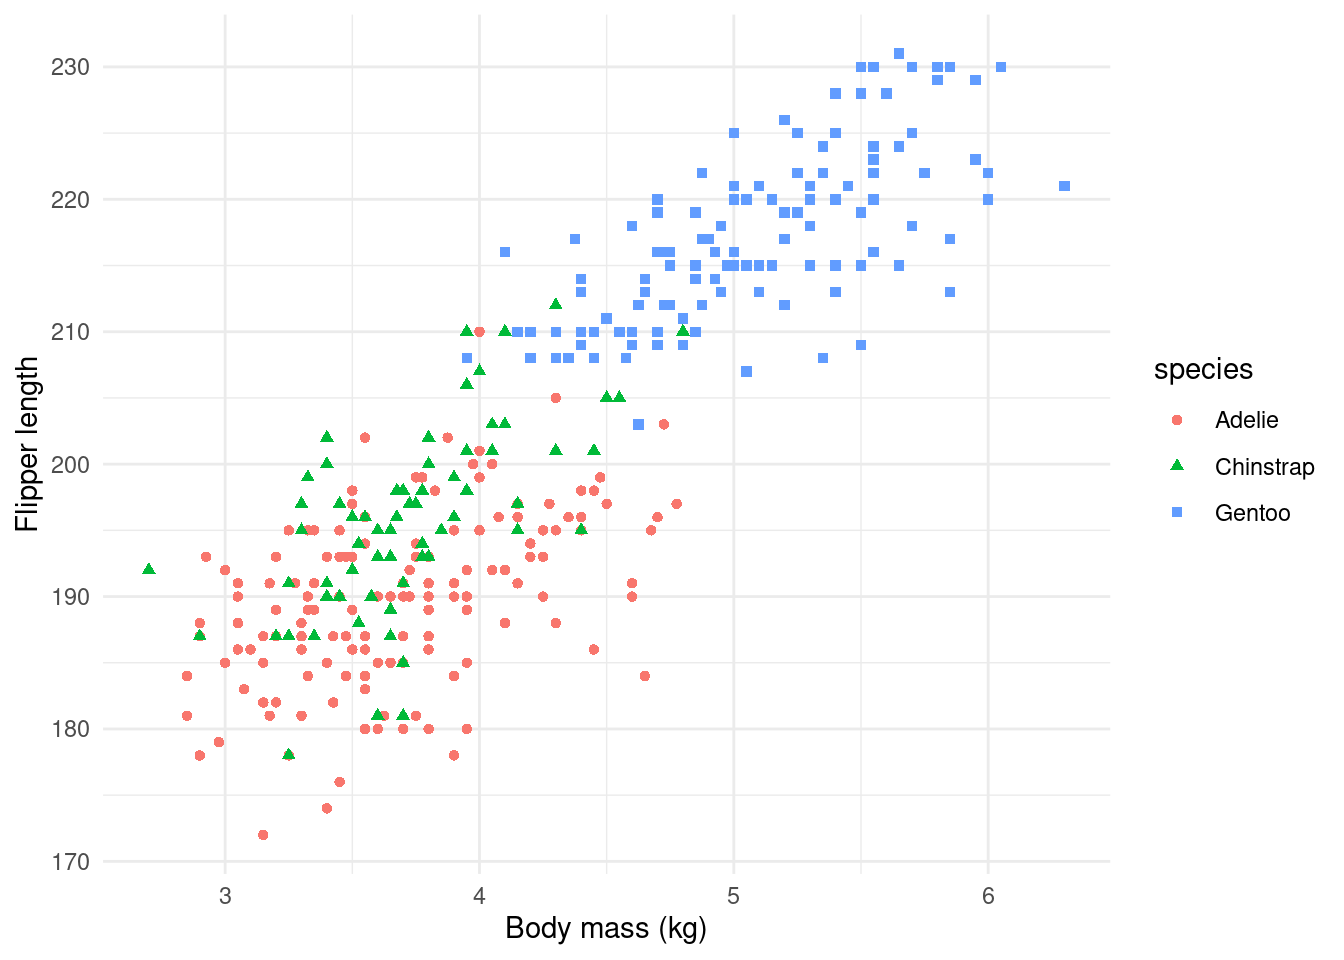
\includegraphics{lecture03---visualization_files/figure-latex/unnamed-chunk-20-1.pdf}

If none of the color palettes work, we can always create our own

\begin{Shaded}
\begin{Highlighting}[]
\NormalTok{kard\_tidy }\SpecialCharTok{\%\textgreater{}\%} 
  \FunctionTok{ggplot}\NormalTok{(}\FunctionTok{aes}\NormalTok{(}\AttributeTok{x =}\NormalTok{ date, }\AttributeTok{y =}\NormalTok{ score, }\AttributeTok{color =}\NormalTok{ name)) }\SpecialCharTok{+}
  \FunctionTok{geom\_line}\NormalTok{() }\SpecialCharTok{+}
  \FunctionTok{labs}\NormalTok{(}\AttributeTok{x =} \StringTok{"Date"}\NormalTok{,}
       \AttributeTok{y =} \StringTok{"Popularity"}\NormalTok{,}
       \AttributeTok{title =} \StringTok{"The Popularity of the Kardashians"}\NormalTok{,}
       \AttributeTok{subtitle =} \StringTok{"Google trends data"}
\NormalTok{       ) }\SpecialCharTok{+}
  \FunctionTok{scale\_color\_manual}\NormalTok{(}\AttributeTok{name =} \StringTok{"Name"}\NormalTok{,}
                     \AttributeTok{labels =} \FunctionTok{c}\NormalTok{(}\StringTok{"Kendall"}\NormalTok{, }\StringTok{"Khloe"}\NormalTok{, }\StringTok{"Kim"}\NormalTok{, }\StringTok{"Kourtney"}\NormalTok{, }\StringTok{"Kylie"}\NormalTok{),}
                     \AttributeTok{values =} \FunctionTok{c}\NormalTok{(}\StringTok{"\#C9D2FF"}\NormalTok{, }\StringTok{"\#F26379"}\NormalTok{, }\StringTok{"\#4B67F2"}\NormalTok{, }\StringTok{"\#F2C333"}\NormalTok{, }\StringTok{"\#3FF262"}\NormalTok{)) }\SpecialCharTok{+}
  \FunctionTok{theme\_classic}\NormalTok{()}
\end{Highlighting}
\end{Shaded}

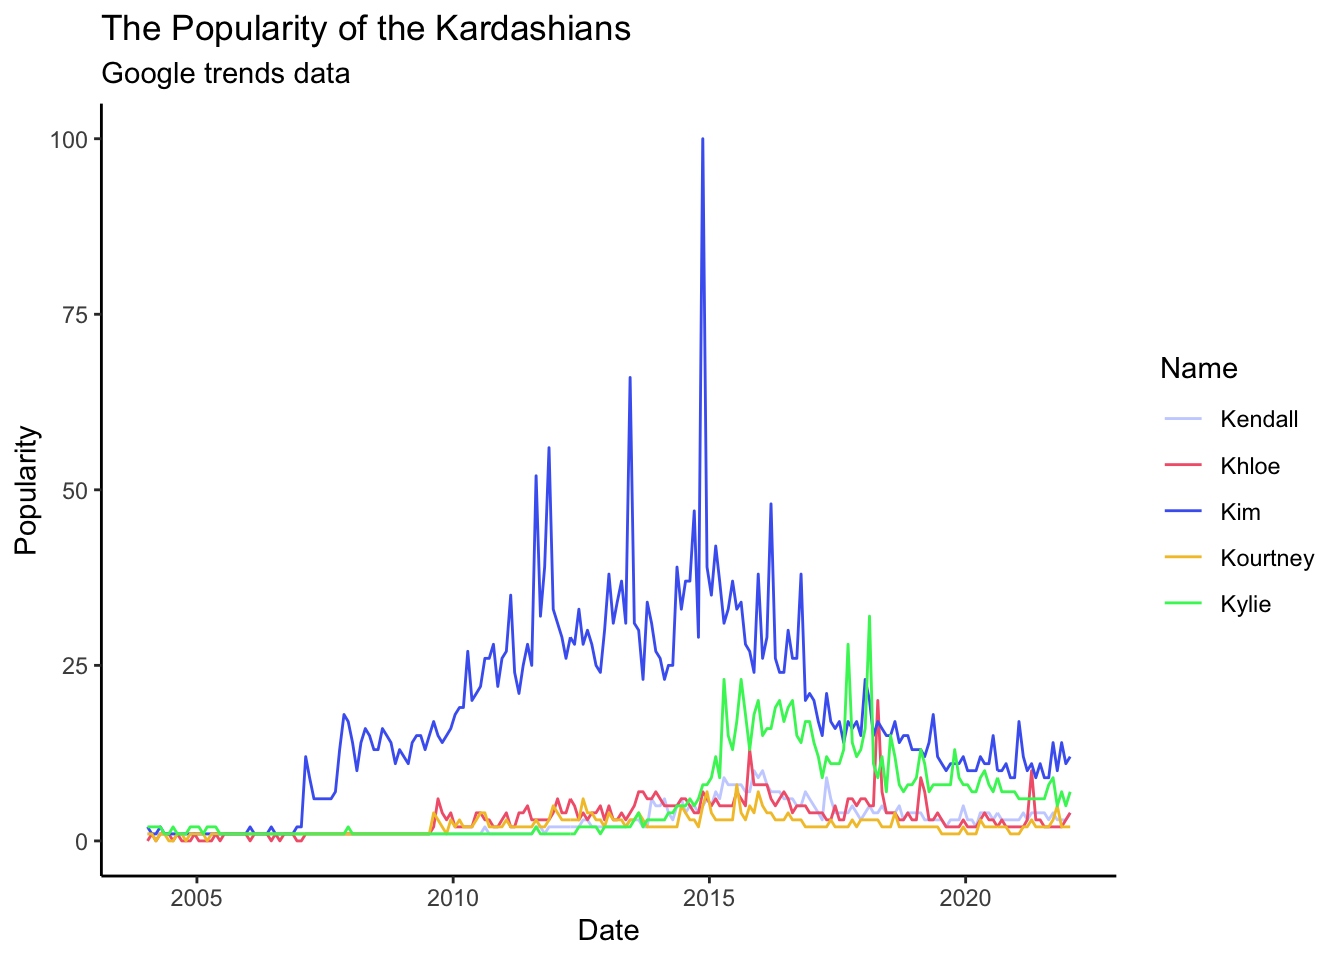
\includegraphics{lecture03---visualization_files/figure-latex/unnamed-chunk-21-1.pdf}

We can also try different aesthetics to see what works better.

\begin{Shaded}
\begin{Highlighting}[]
\NormalTok{kard\_tidy }\SpecialCharTok{\%\textgreater{}\%} 
  \FunctionTok{ggplot}\NormalTok{(}\FunctionTok{aes}\NormalTok{(}\AttributeTok{x =}\NormalTok{ date, }\AttributeTok{y =}\NormalTok{ score, }\AttributeTok{color =}\NormalTok{ name)) }\SpecialCharTok{+}
  \FunctionTok{geom\_point}\NormalTok{() }\SpecialCharTok{+}
  \FunctionTok{labs}\NormalTok{(}\AttributeTok{x =} \StringTok{"Date"}\NormalTok{,}
       \AttributeTok{y =} \StringTok{"Popularity"}\NormalTok{,}
       \AttributeTok{title =} \StringTok{"The Popularity of the Kardashians"}\NormalTok{,}
       \AttributeTok{subtitle =} \StringTok{"Google trends data"}
\NormalTok{       ) }\SpecialCharTok{+}
  \FunctionTok{scale\_color\_lancet}\NormalTok{(}\AttributeTok{name =} \StringTok{"Name"}\NormalTok{,}
                     \AttributeTok{labels =} \FunctionTok{c}\NormalTok{(}\StringTok{"Kendall"}\NormalTok{, }\StringTok{"Khloe"}\NormalTok{, }\StringTok{"Kim"}\NormalTok{, }\StringTok{"Kourtney"}\NormalTok{, }\StringTok{"Kylie"}\NormalTok{)}
\NormalTok{                       ) }\SpecialCharTok{+}
  \FunctionTok{theme\_classic}\NormalTok{()}
\end{Highlighting}
\end{Shaded}

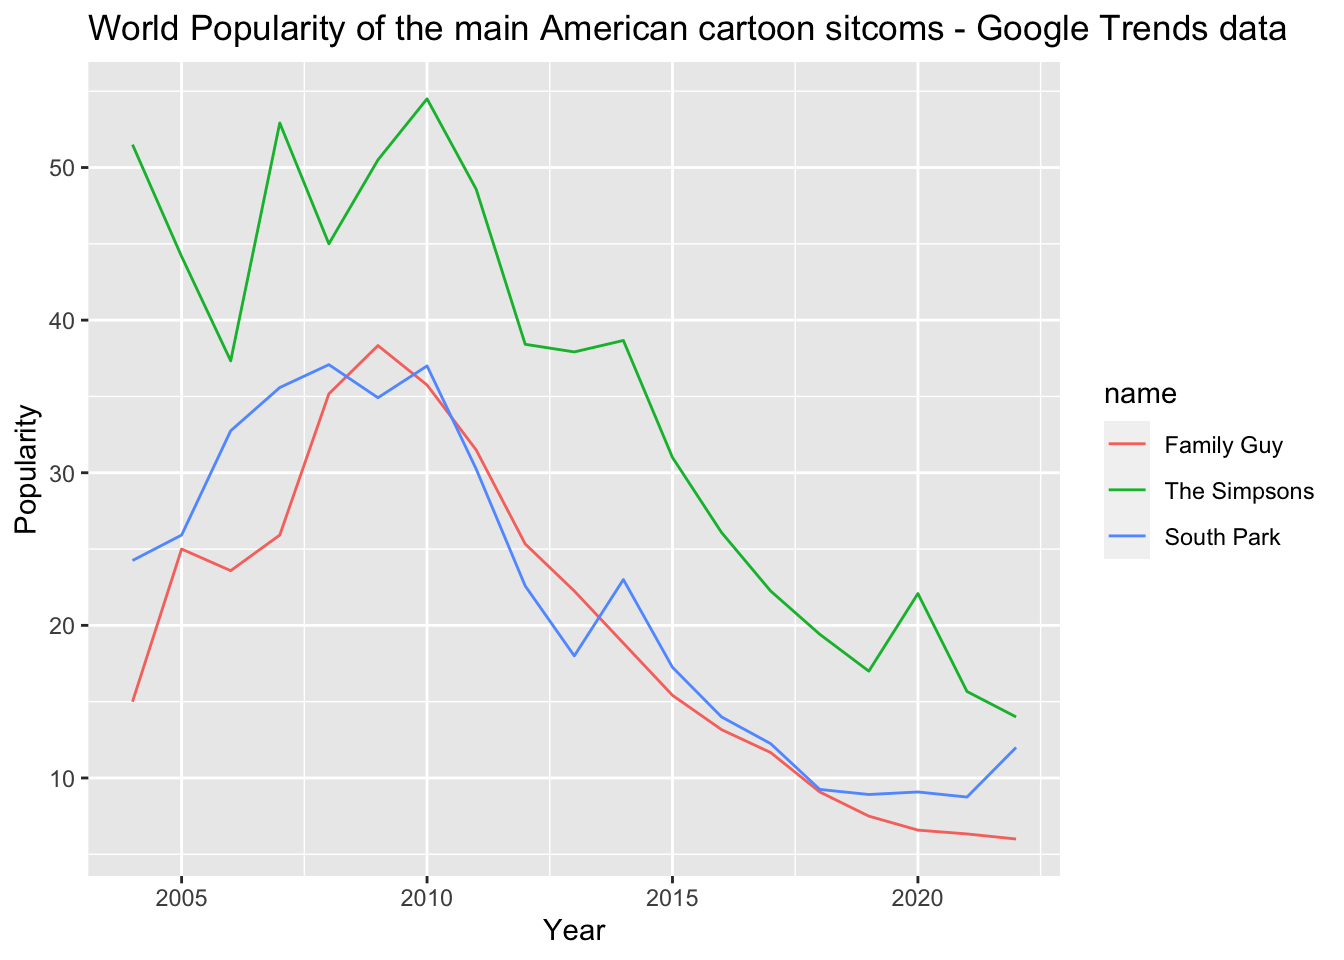
\includegraphics{lecture03---visualization_files/figure-latex/unnamed-chunk-22-1.pdf}

\begin{Shaded}
\begin{Highlighting}[]
\NormalTok{kard\_tidy }\SpecialCharTok{\%\textgreater{}\%} 
  \FunctionTok{ggplot}\NormalTok{(}\FunctionTok{aes}\NormalTok{(}\AttributeTok{x =}\NormalTok{ date, }\AttributeTok{y =}\NormalTok{ score, }\AttributeTok{color =}\NormalTok{ name, }\AttributeTok{fill =}\NormalTok{ name)) }\SpecialCharTok{+}
  \FunctionTok{geom\_col}\NormalTok{() }\SpecialCharTok{+}
  \FunctionTok{labs}\NormalTok{(}\AttributeTok{x =} \StringTok{"Date"}\NormalTok{,}
       \AttributeTok{y =} \StringTok{"Popularity"}\NormalTok{,}
       \AttributeTok{title =} \StringTok{"The Popularity of the Kardashians"}\NormalTok{,}
       \AttributeTok{subtitle =} \StringTok{"Google trends data"}
\NormalTok{       ) }\SpecialCharTok{+}
  \FunctionTok{scale\_fill\_lancet}\NormalTok{(}\AttributeTok{name =} \StringTok{"Name"}\NormalTok{,}
                     \AttributeTok{labels =} \FunctionTok{c}\NormalTok{(}\StringTok{"Kendall"}\NormalTok{, }\StringTok{"Khloe"}\NormalTok{, }\StringTok{"Kim"}\NormalTok{, }\StringTok{"Kourtney"}\NormalTok{, }\StringTok{"Kylie"}\NormalTok{)}
\NormalTok{                       ) }\SpecialCharTok{+}
  \FunctionTok{scale\_color\_discrete}\NormalTok{(}\AttributeTok{guide =} \StringTok{"none"}\NormalTok{) }\SpecialCharTok{+}
  \FunctionTok{theme\_classic}\NormalTok{()}
\end{Highlighting}
\end{Shaded}

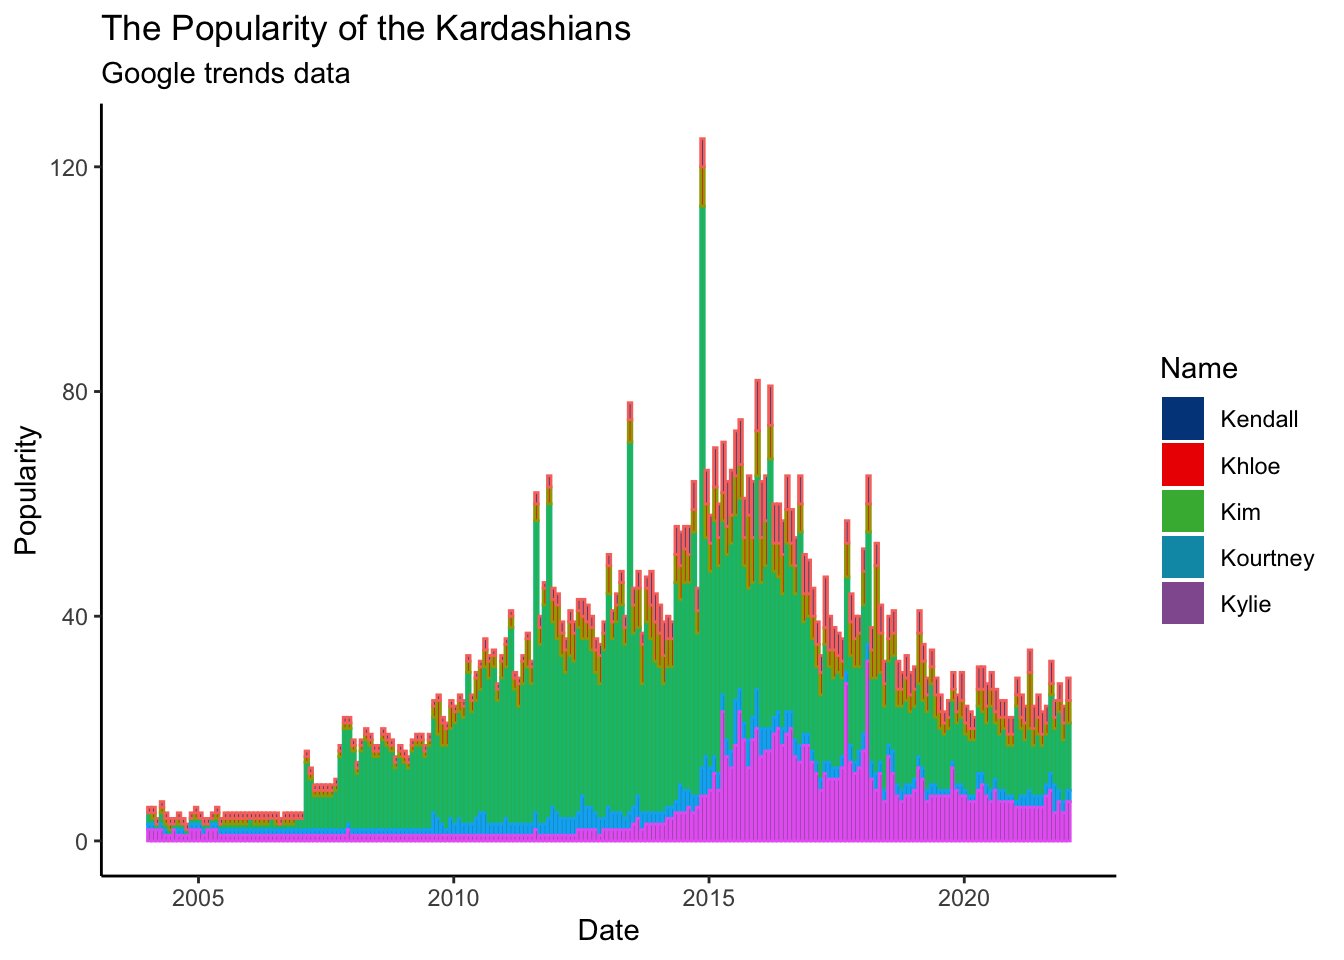
\includegraphics{lecture03---visualization_files/figure-latex/unnamed-chunk-23-1.pdf}

\begin{Shaded}
\begin{Highlighting}[]
\NormalTok{kard\_tidy }\SpecialCharTok{\%\textgreater{}\%} 
  \FunctionTok{group\_by}\NormalTok{(month, name) }\SpecialCharTok{\%\textgreater{}\%} 
  \FunctionTok{summarize}\NormalTok{(}\AttributeTok{mean\_score =} \FunctionTok{mean}\NormalTok{(score)) }\SpecialCharTok{\%\textgreater{}\%} 
  \FunctionTok{ggplot}\NormalTok{(}\FunctionTok{aes}\NormalTok{(}\AttributeTok{x =}\NormalTok{ month, }\AttributeTok{y =}\NormalTok{ mean\_score, }\AttributeTok{fill =}\NormalTok{ name)) }\SpecialCharTok{+}
  \FunctionTok{geom\_col}\NormalTok{(}\AttributeTok{position =} \StringTok{"dodge"}\NormalTok{, }\AttributeTok{alpha =} \DecValTok{0}\NormalTok{) }\SpecialCharTok{+}
  \FunctionTok{geom\_point}\NormalTok{() }\SpecialCharTok{+}
  \FunctionTok{geom\_polygon}\NormalTok{(}\AttributeTok{alpha =} \FloatTok{0.2}\NormalTok{) }\SpecialCharTok{+} 
  \FunctionTok{scale\_x\_continuous}\NormalTok{(}\AttributeTok{breaks =} \DecValTok{1}\SpecialCharTok{:}\DecValTok{12}\NormalTok{, }\AttributeTok{labels =}\NormalTok{  month.abb[}\DecValTok{1}\SpecialCharTok{:}\DecValTok{12}\NormalTok{]) }\SpecialCharTok{+} 
  \FunctionTok{coord\_polar}\NormalTok{()}
\end{Highlighting}
\end{Shaded}

\begin{verbatim}
## `summarise()` has grouped output by 'month'. You can override using the `.groups` argument.
\end{verbatim}

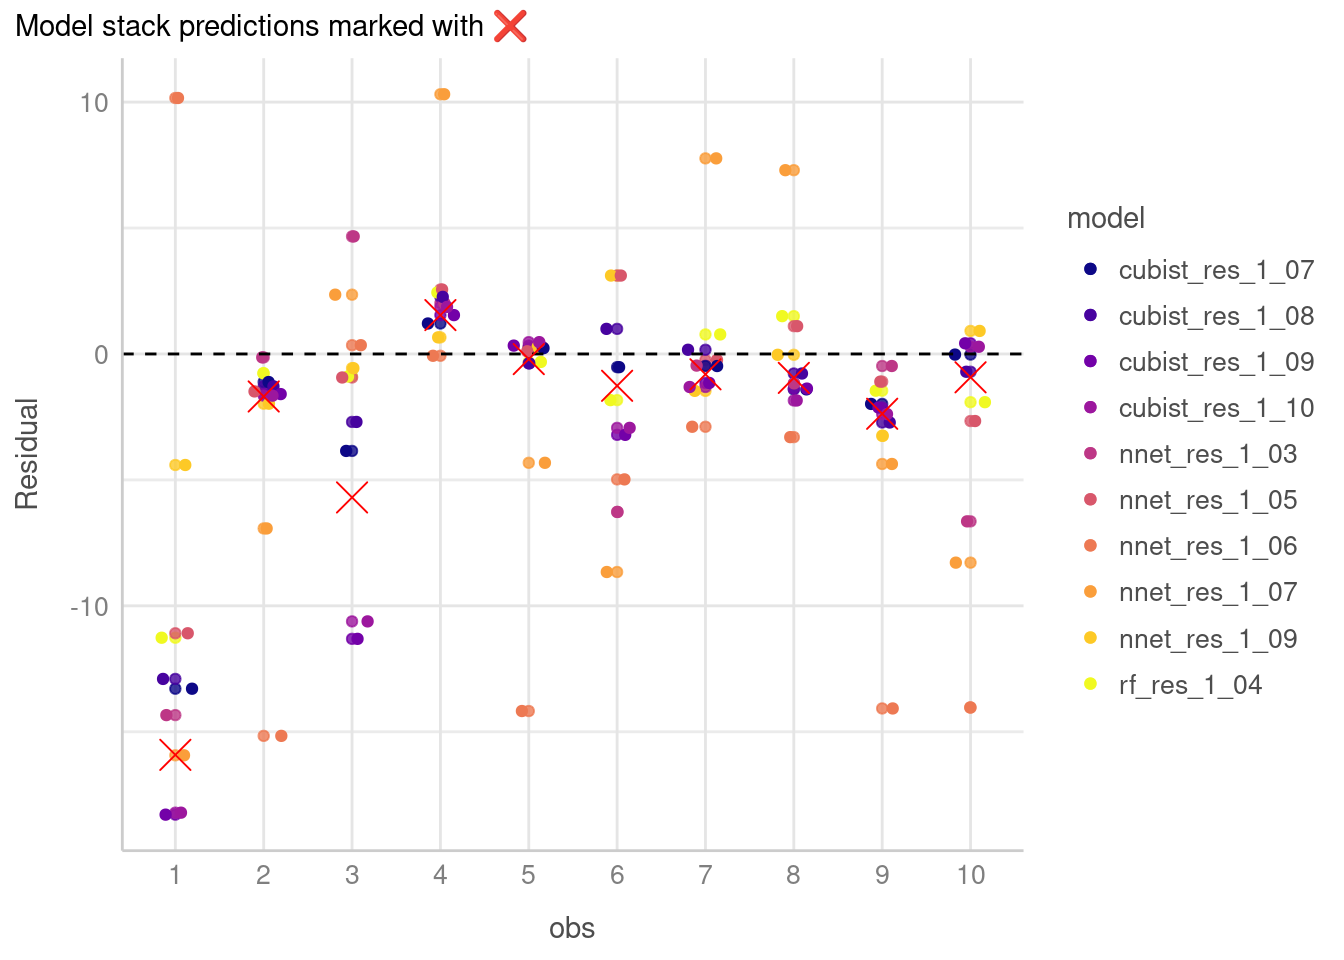
\includegraphics{lecture03---visualization_files/figure-latex/unnamed-chunk-24-1.pdf}

Maps are nothing more than just graphs, too We can load the map of the
US

\begin{Shaded}
\begin{Highlighting}[]
\FunctionTok{library}\NormalTok{(usmap)}
\end{Highlighting}
\end{Shaded}

and use it to plot the popularity of search terms by state

\begin{Shaded}
\begin{Highlighting}[]
\FunctionTok{plot\_usmap}\NormalTok{(}\AttributeTok{regions =} \StringTok{"states"}\NormalTok{)}
\end{Highlighting}
\end{Shaded}

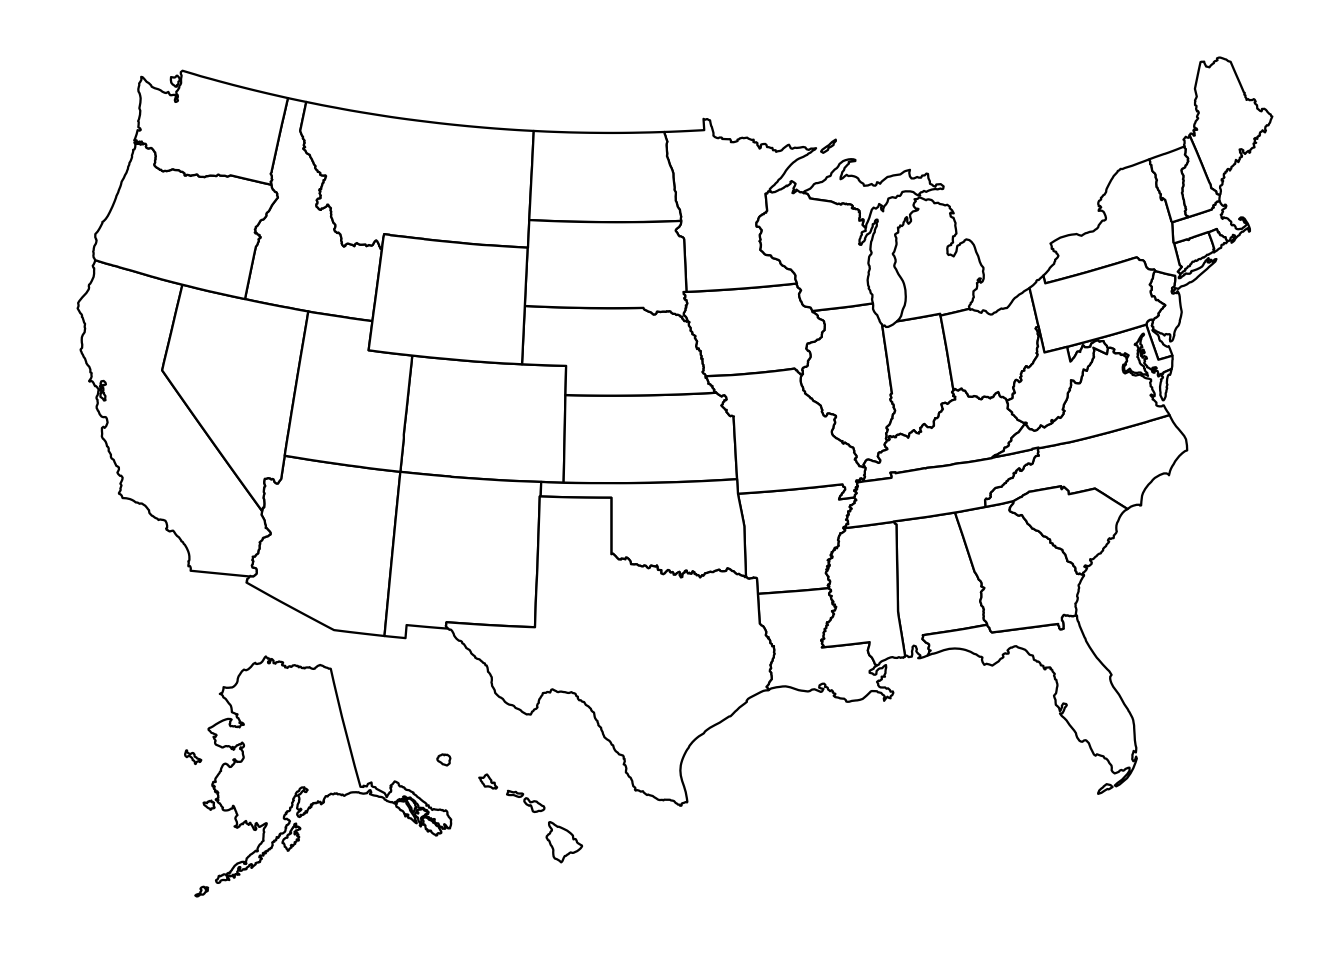
\includegraphics{lecture03---visualization_files/figure-latex/unnamed-chunk-26-1.pdf}

\begin{Shaded}
\begin{Highlighting}[]
\NormalTok{wawa }\OtherTok{\textless{}{-}} \FunctionTok{read\_csv}\NormalTok{(}\StringTok{"geoMap.csv"}\NormalTok{, }\AttributeTok{skip =} \DecValTok{1}\NormalTok{)}
\end{Highlighting}
\end{Shaded}

\begin{verbatim}
## Rows: 51 Columns: 2
\end{verbatim}

\begin{verbatim}
## -- Column specification ---------------------------------------------------------------------------------------
## Delimiter: ","
## chr (1): Region
## dbl (1): Wawa: (1/1/04 - 1/27/22)
\end{verbatim}

\begin{verbatim}
## 
## i Use `spec()` to retrieve the full column specification for this data.
## i Specify the column types or set `show_col_types = FALSE` to quiet this message.
\end{verbatim}

\begin{Shaded}
\begin{Highlighting}[]
\NormalTok{wawa\_clean }\OtherTok{\textless{}{-}}\NormalTok{ wawa }\SpecialCharTok{\%\textgreater{}\%} \FunctionTok{rename}\NormalTok{(}\AttributeTok{state =}\NormalTok{ Region,}
                \AttributeTok{wawa =} \StringTok{\textasciigrave{}}\AttributeTok{Wawa: (1/1/04 {-} 1/27/22)}\StringTok{\textasciigrave{}}\NormalTok{) }\SpecialCharTok{\%\textgreater{}\%} 
  \FunctionTok{mutate}\NormalTok{(}\AttributeTok{fips =} \FunctionTok{fips}\NormalTok{(state))}
  
\FunctionTok{plot\_usmap}\NormalTok{(}\AttributeTok{data =}\NormalTok{ wawa\_clean, }\AttributeTok{regions =} \StringTok{"states"}\NormalTok{, }\AttributeTok{values =} \StringTok{"wawa"}\NormalTok{) }\SpecialCharTok{+}
\FunctionTok{scale\_fill\_viridis\_c}\NormalTok{()}
\end{Highlighting}
\end{Shaded}

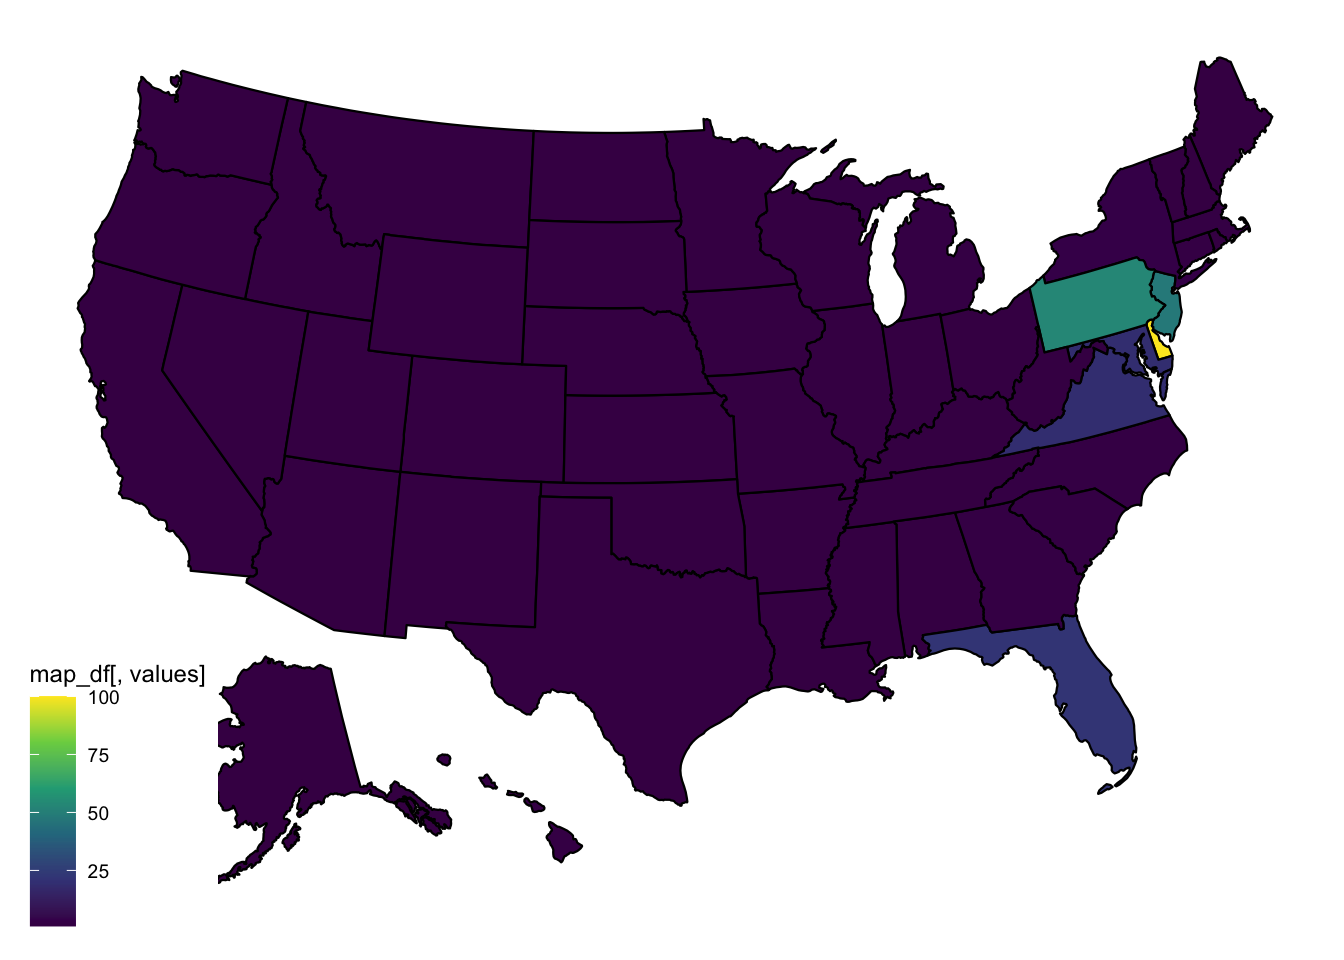
\includegraphics{lecture03---visualization_files/figure-latex/unnamed-chunk-27-1.pdf}

\end{document}
